\chapter{用巨洞探测重子声波振荡信号}
\label{cha:voidbao}
%%%%%%%%%%%%%%%%%%%%%%%%%%%%%%

\section{引言}

第~\ref{cha:DIVE} 章介绍了巨洞的一些统计性质,根据巨洞这些统计性质的研究就可以推测半径大于16 $h^{-1}$ Mpc的DT巨洞能被认为是真正宇宙学意义上的巨洞。在本章巨洞成团性的研究中我们仍然会使用一部分半径小于16 $h^{-1}$ Mpc的巨洞来展示不同半径大小的DT巨洞在成团性上的区别。

根据半径将DT巨洞分成许多组子样本,然后计算这些巨洞子样本的中心位置的自相关函数(auto-correlation function)和不同子样本与星系或暗物质晕的互相关函数(cross-correlation function)。先使用完整实空间模拟暗物质晕表研究不同巨洞子样本BAO信号的显著性,为了快速测量不同子样本的BAO信号的显著性,我们引入了一个估计BAO信号信噪比(signal-to-noise ratio,$S/N$)的方法。然后研究了红移空间完整模拟暗物质晕表内巨洞的BAO显著性与实空间结果的差异。接下来使用模拟光锥星系表研究不同巨洞子样本BAO信号显著性的变化。综合以上三组数据的结果选出最佳的巨洞子样本,并计算BOSS/SDSS-III CMASS DR11
%和DR12
观测数据对应的巨洞子样本的BAO显著性,这时我们使用了第~\ref{sec:isobao} 章介绍的测量BAO特征尺度的方法。

\section{巨洞在完整模拟暗物质晕表里的BAO信号}
\label{sec:voidbaocomplete}

\begin{figure}
\centering
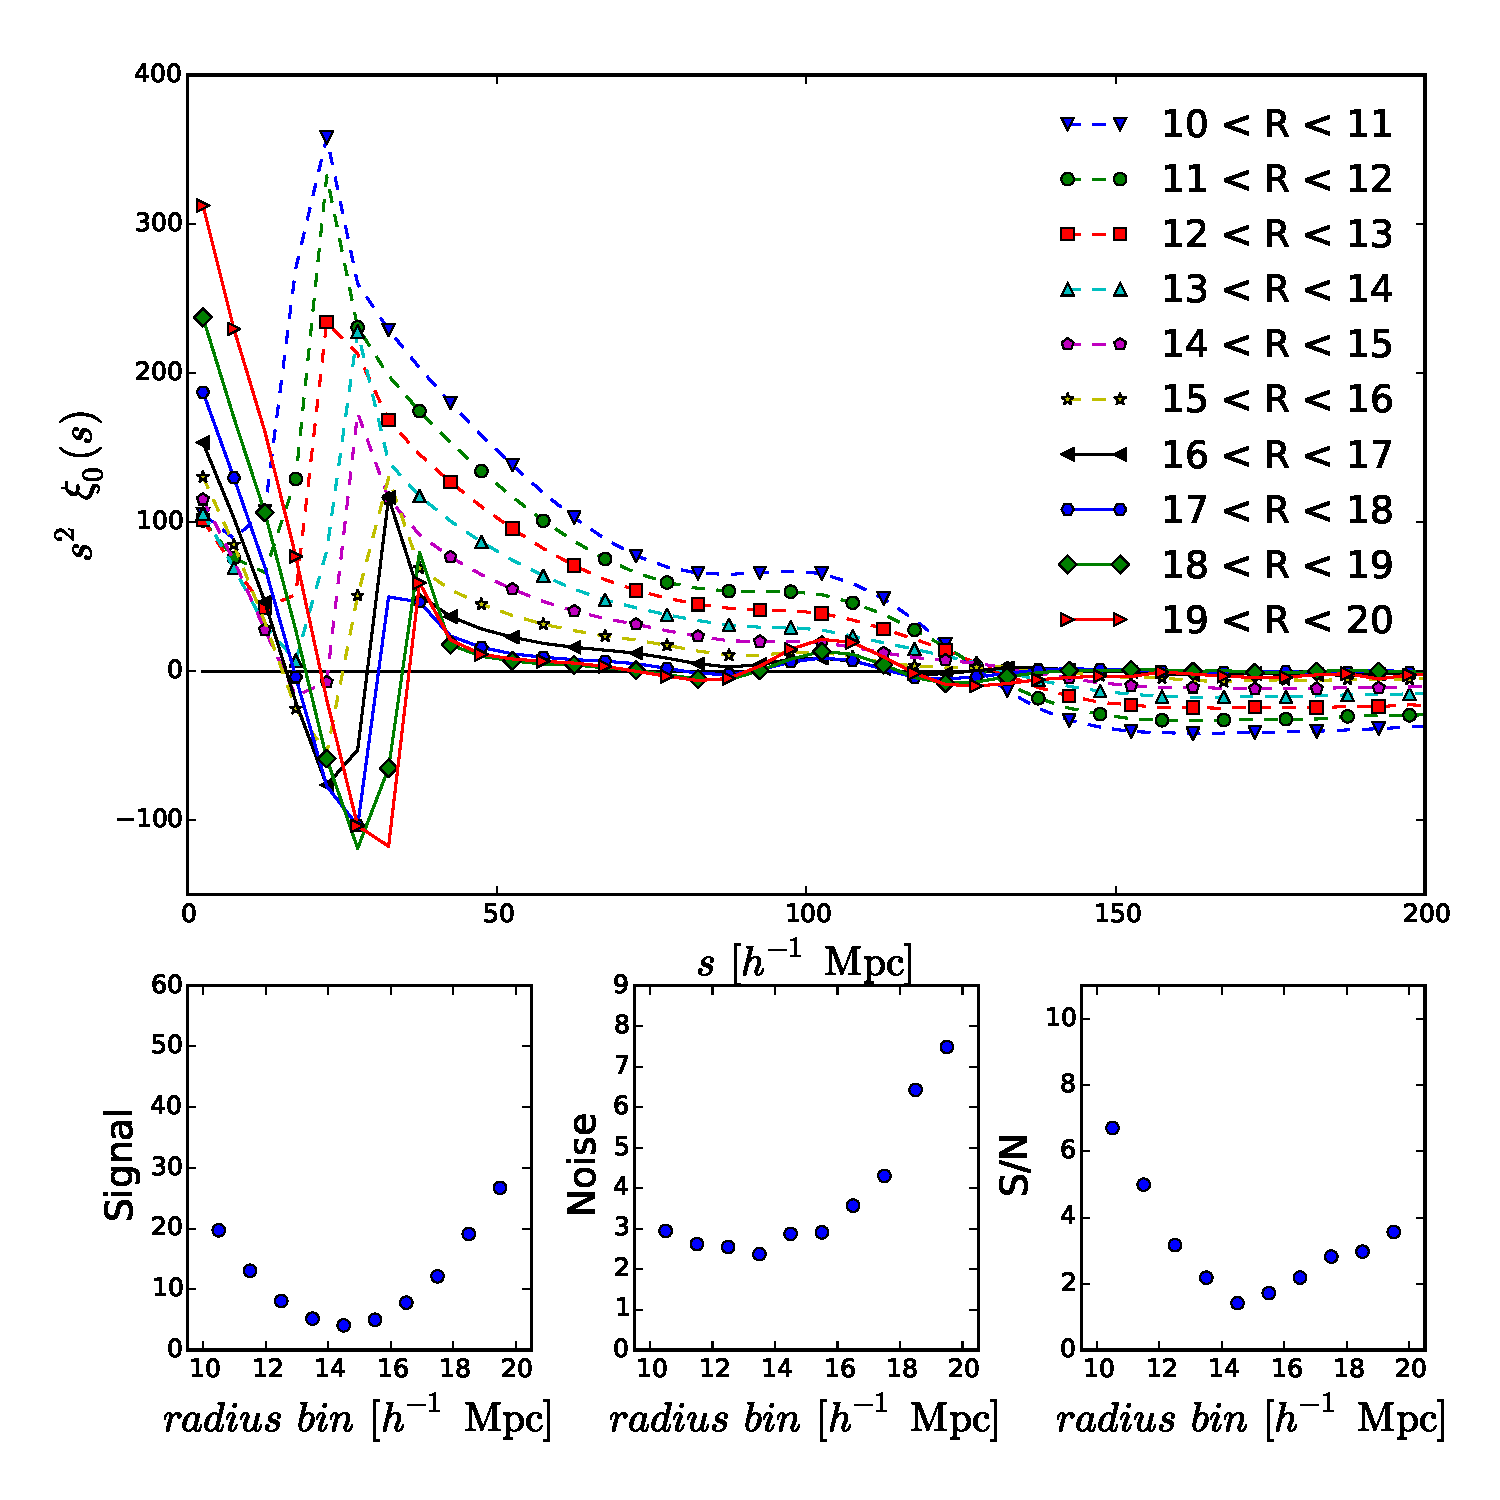
\includegraphics[width=.9\textwidth]{cf_box_r_bins_real_space_2015_11_13_all.pdf}
\caption{在红移$z = 0.56$处,100个实空间完整模拟暗物质晕表通过DIVE得到的不同半径区间$R_1 < R < R_2$(radius bin)的巨洞的平均2PCF(上图),和用第~\ref{sec:sn} 章测量BAO信号信噪比方法得到的$S$,$N$和$S/N$(下图)。(文献 ~\inlinecite{Liang2016}中的Figure 1)}
\label{fig:cf_box_r_bins_real_space}
\end{figure}

\begin{figure}
\centering
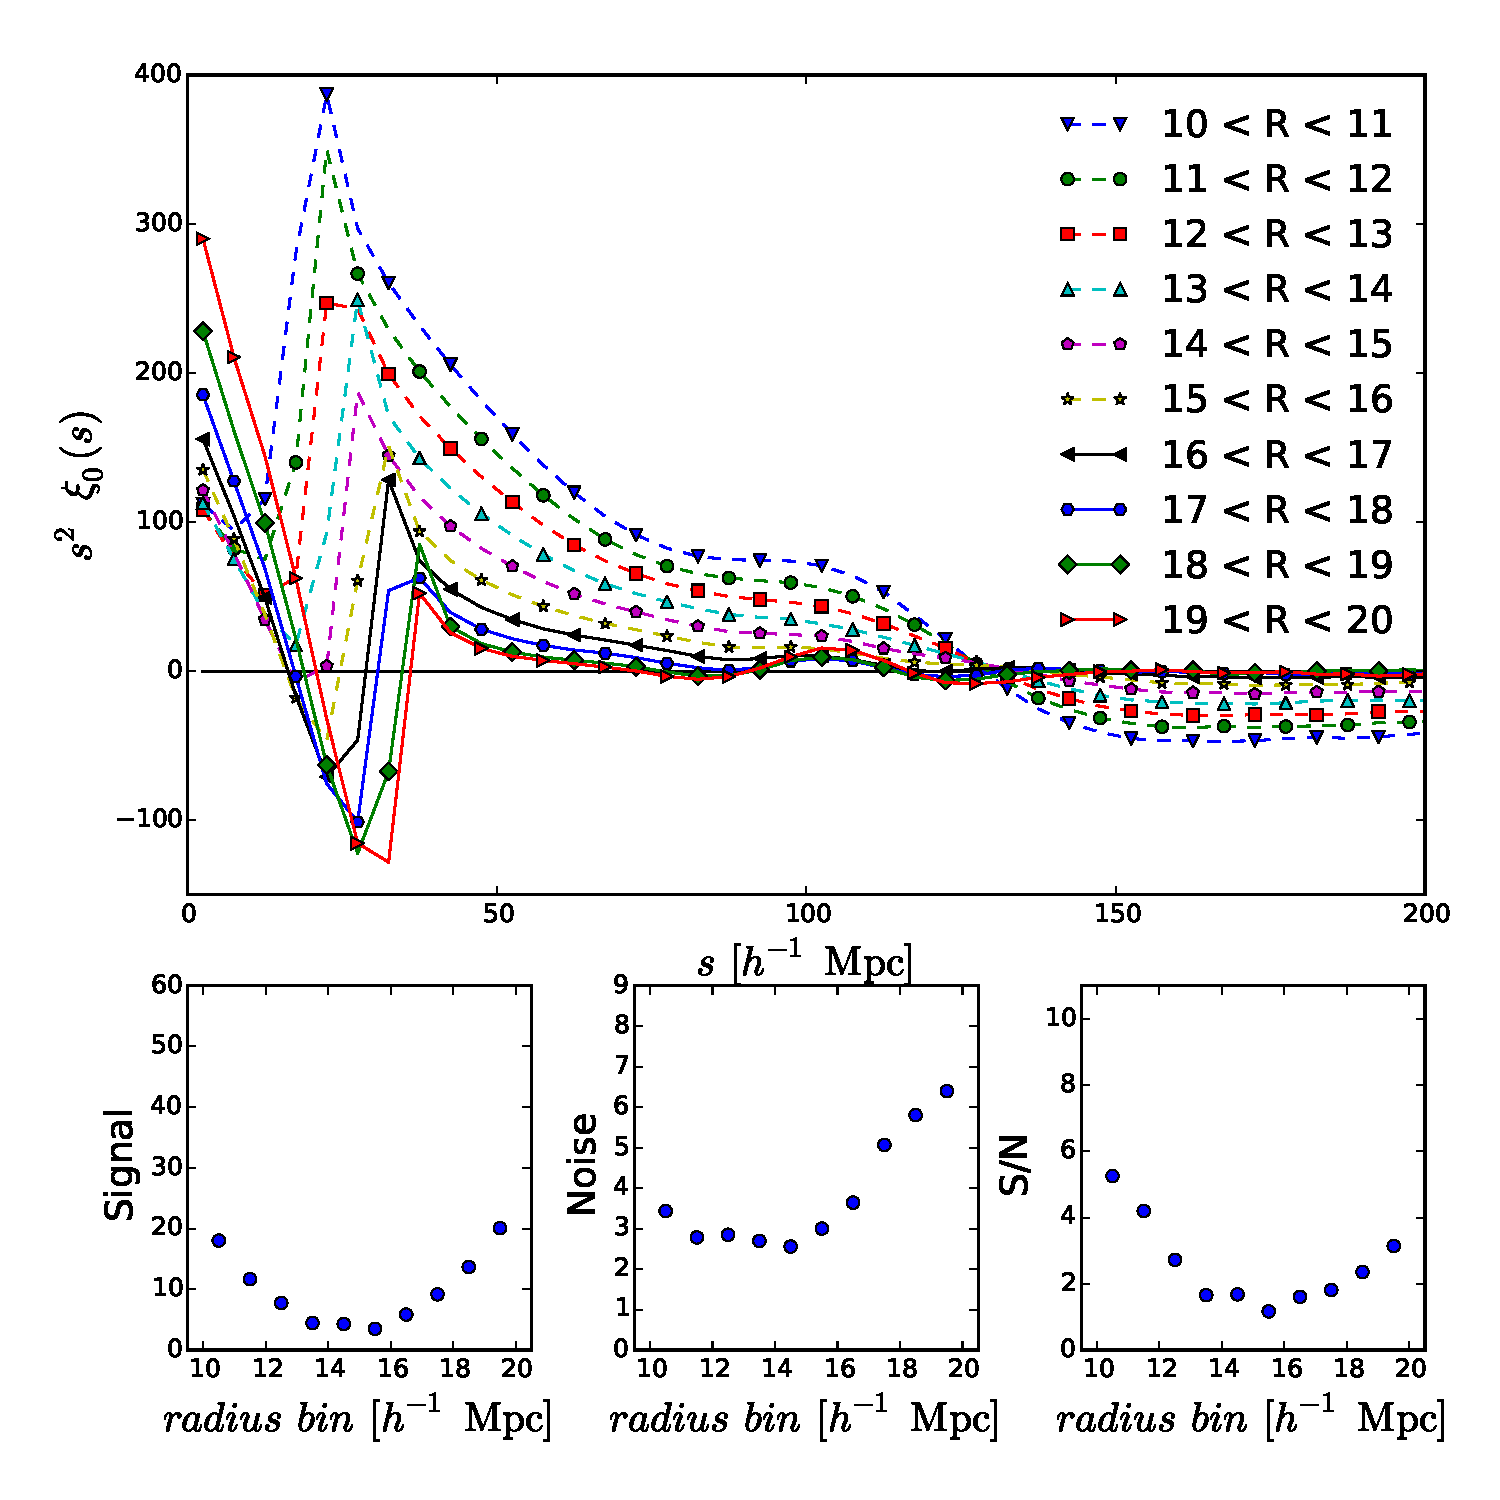
\includegraphics[width=.9\textwidth]{cf_box_r_bins_redshift_space_2015_11_13_all.pdf}
\caption{在红移$z = 0.56$处,100个红移空间完整模拟暗物质晕表通过DIVE得到的不同半径区间$R_1 < R < R_2$的巨洞的平均2PCF(上图),和用第~\ref{sec:sn} 章测量BAO信号信噪比方法得到的$S$,$N$和$S/N$(下图)。(文献 ~\inlinecite{Liang2016}中的Figure 2)}
\label{fig:cf_box_r_bins_redshift_space}
\end{figure}

\begin{figure}
\centering
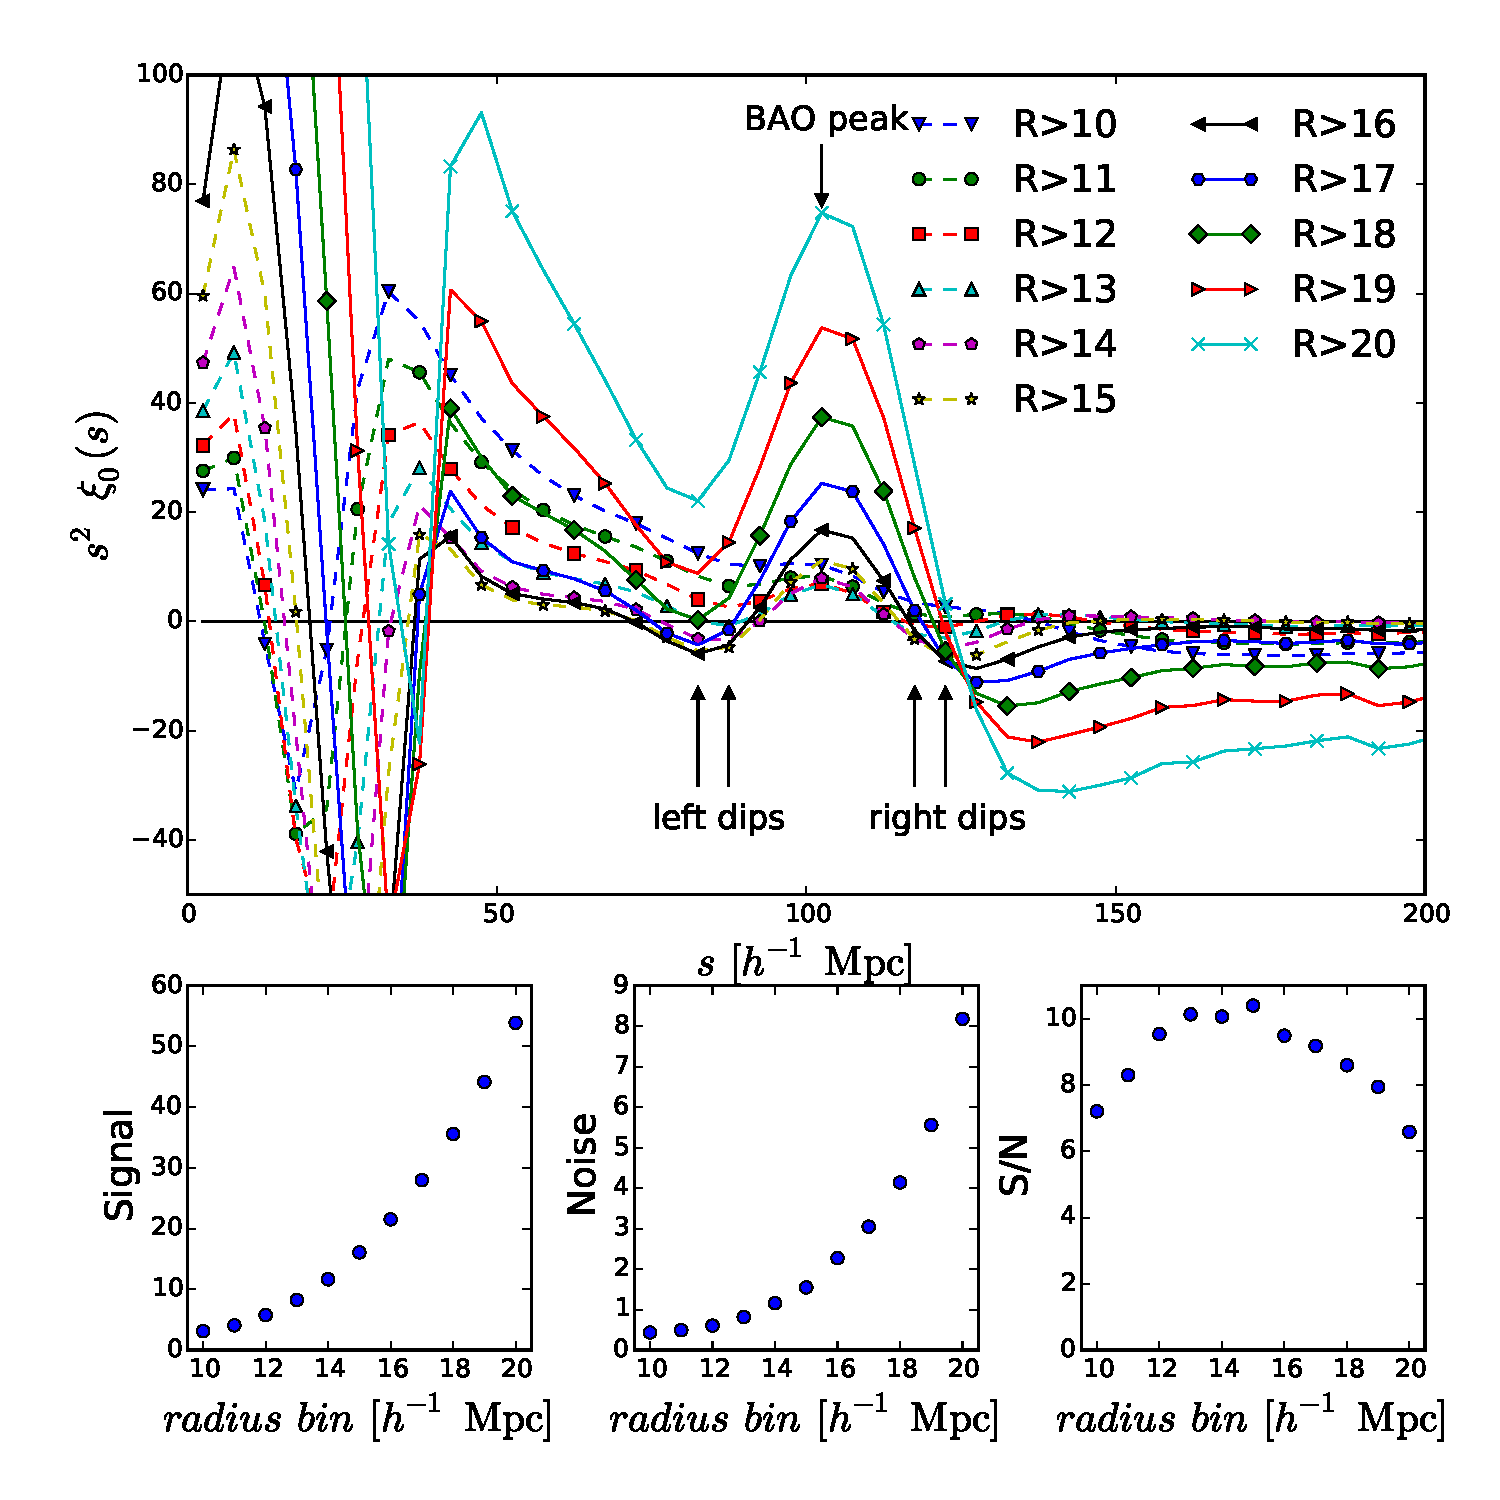
\includegraphics[width=.9\textwidth]{cf_box_r_cuts_real_space_2015_11_13.pdf}
\caption{在红移$z = 0.56$处,100个实空间完整模拟暗物质晕表通过DIVE得到的不同最小半径$R > R_{cut}$的巨洞的平均2PCF(上图),和用第~\ref{sec:sn} 章测量BAO信号信噪比方法得到的$S$,$N$和$S/N$(下图)。图中箭头标记了BAO信号信噪比时BAO特征尺度(BAO peak)和其左右两边所对应的低谷(left dips、right dips)的位置。(文献 ~\inlinecite{Liang2016}中的Figure 1)}
\label{fig:cf_box_r_cuts_real_space}
\end{figure}

\begin{figure}
\centering
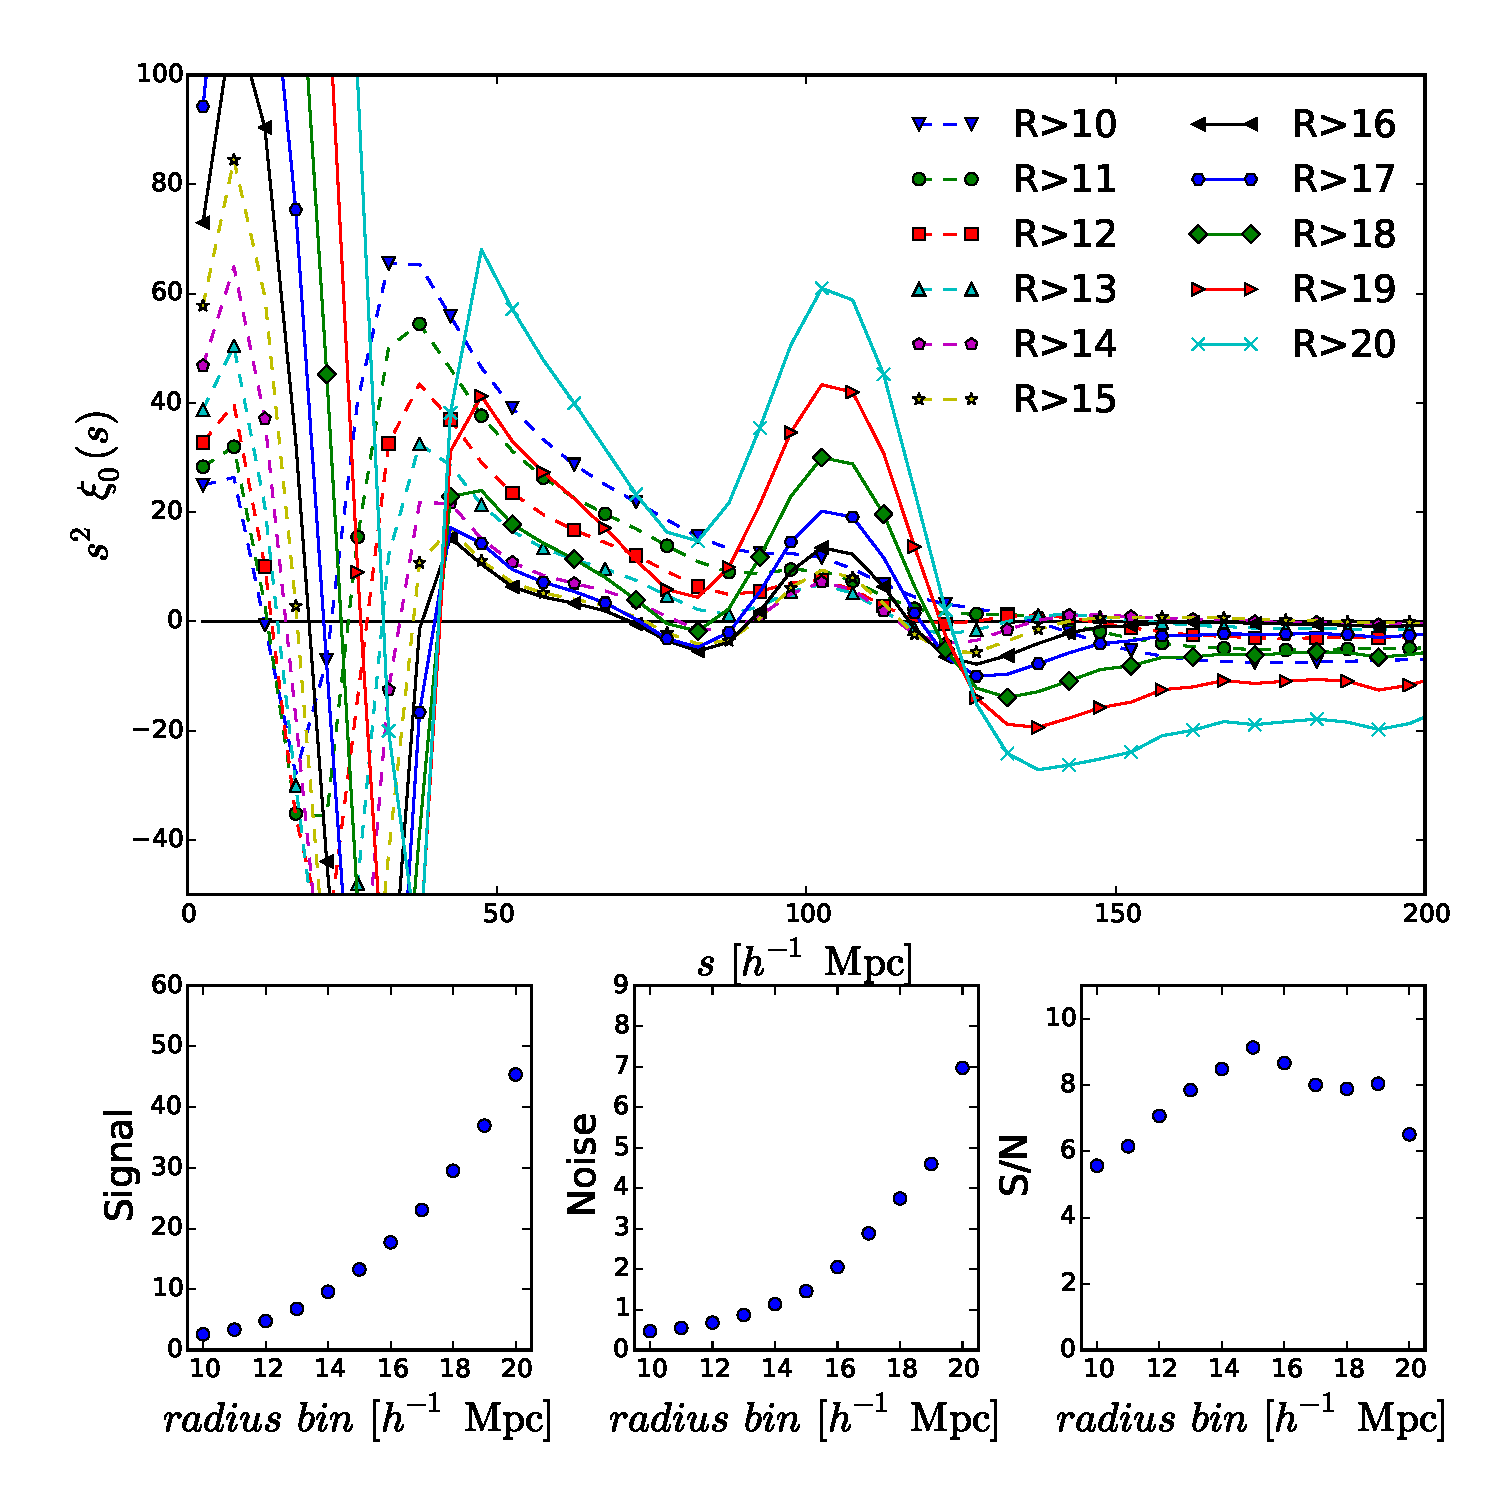
\includegraphics[width=.9\textwidth]{cf_box_r_cuts_redshift_space_2015_11_13.pdf}
\caption{在红移$z = 0.56$处,100个红移空间完整模拟暗物质晕表通过DIVE得到的不同最小半径$R > R_{cut}$的巨洞的平均2PCF(上图),和用第~\ref{sec:sn} 章测量BAO信号信噪比方法得到的$S$,$N$和$S/N$(下图)。(文献 ~\inlinecite{Liang2016}中的Figure 2)}
\label{fig:cf_box_r_cuts_redshift_space}
\end{figure}

\subsection{测量完整模拟暗物质晕表内巨洞的2PCF}

我们采取第~\ref{cha:DIVE} 章中介绍的方法用DIVE得到完整模拟暗物质晕表的巨洞数据。通过计算巨洞中心位置的2PCF,$\xi(s)$,来测量BAO信号。在本文的所有2PCF相关的图中为了使BAO信号看上去更加明显,纵轴的数值都采用的是$s^2 \xi(s)$。

因为完整模拟暗物质晕表是在具有周期性边界条件的立方体盒子中,这时估算2PCF的式子中,表示随机样本对数的$RR$项可以由解析表达式精确的计算得出。所以我们用使用The Peebles \& Hauser Estimator~\cite{Peebles1974}
\begin{equation}
\xi (s)=\frac {DD(s)} {RR(s)} - 1
\end{equation}
来估算2PCF。其中$RR$项可以用
\begin{equation}
RR(s) = \frac{4\pi}{3}  \frac {s_{\rm max}^3 - s_{\rm min}^3}{2V}\,,
\end{equation}
直接精确计算。$V$是立方体盒子的体积。$RR(s)$是从$s_{\rm min}$到$s_{\rm max}$这个距离区间内随机样本对数归一化后的数值,$s$的值一般取为
$
s = (s_{\rm max} + s_{\rm min})/2
$。

图~\ref{fig:cf_box_r_bins_real_space} 是实空间完整模拟暗物质晕表的不同半径区间[$R_1$,$R_2$]内巨洞的2PCF,图~\ref{fig:cf_box_r_bins_redshift_space} 是红移空间完整模拟暗物质晕表的对应结果。

\subsection{不依赖具体模型的估计BAO信号显著性的方法}
\label{sec:sn}

从图~\ref{fig:cf_box_r_bins_real_space} 和图~\ref{fig:cf_box_r_bins_redshift_space} 中可以看到,巨洞所有子样本的2PCF都在略小于两倍半径的距离上出现很强的负相关。这是由巨洞排斥效应(void exclusion effect)造成的~\cite{Hamaus2014}。

BAO信号的峰值出现在$\sim$102.5  $h^{-1}$ Mpc,这一特征可以在半径大于16 $h^{-1}$ Mpc的巨洞子样本的2PCF结果中清晰的识别。在BAO信号峰值位置$\sim$102.5  $h^{-1}$ Mpc的两边,$\sim$85  $h^{-1}$ Mpc和$\sim$120  $h^{-1}$ Mpc处存在两个局部的低谷。图~\ref{fig:cf_box_r_bins_real_space}和图~\ref{fig:cf_box_r_bins_redshift_space} 中在半径区间$17<R<18$到$19<R<20$ $h^{-1}$ Mpc和图~\ref{fig:cf_box_r_cuts_real_space} 和图~\ref{fig:cf_box_r_cuts_redshift_space} 中半径大于$R>13$  $h^{-1}$ Mpc的巨洞子样本的2PCF可以较明显看到这两个低谷的形状和位置。这一特征在星系或暗物质晕的2PCF中并不明显,而我们利用巨洞2PCF的这一特征创造性的引入了一个不依赖宇宙学模型的估计BAO信号信噪比的方法。
%{\color{red} Fig.1 in Kitaura et al. (companion paper) shows  the BAO signal obtained as the difference between the correlation function with a simulation without BAO wiggles and  a simulation with BAO wiggles. The peak and dips of the BAO signal are better defined than with the direct 2 point correlation functions. We actually tried several values and several signal definitions. For clarity sake in this paper, we choose to present the results with the definition which gives the highest S/N.}
巨洞的BAO信号$S$定义为:
\begin{equation}
S\equiv \xi(s^{\rm BAO}) - \frac{\xi(s_{\rm 1}^{\rm dl})+\xi(s_{\rm 2}^{\rm dl})+\xi(s_{\rm 1}^{\rm dr})+\xi(s_{\rm 2}^{\rm dr})}{4}
\end{equation}
其中$s^{\rm BAO}=102.5$,$s_{\rm 1}^{\rm dl}=82.5$,$s_{\rm 2}^{\rm dl}=87.5$,$s_{\rm 1}^{\rm dr}=117.5$,$s_{\rm 2}^{\rm dr}=122.5$  { { $h^{-1}$ Mpc}。
$s_{\rm 1}^{\rm dl}$和$s_{\rm 2}^{\rm dl}$对应于BAO峰值左边低谷的位置,$s_{\rm 1}^{\rm dr}$和$s_{\rm 2}^{\rm dr}$对应BAO峰值位置右边低谷的位置。BAO峰值和左右两个低谷的位置都在图~\ref{fig:cf_box_r_cuts_real_space} 中有标注。上标“dl”表示左边的低谷(dip left),上标“dr”表示右边的低谷(dip right)。
%Note that in Kitaura et al. 2015 (companion paper), we use the mock void catalogues to construct the model for measuring BAO with a Markov Chain Monte Carlo analysis. 
尽管这种估计BAO信号的方式有一些主管选择的成分,但是它是自洽的,并且可以非常简单快捷的估计BAO信号的信噪比,不依赖于具体的宇宙学模型。第~\ref{sec:isobao} 章介绍的测量BAO特征尺度的方法进行一次测量至少需要3个小时。所以我们引入的这个方法非常适合用于研究大量不同的巨洞子样本的BAO信号的显著性。BAO信号的噪声$N$被定义为所有用模拟暗物质晕表或模拟星系表测得的$S$的标准差
\begin{equation}
N = \sum^{N_m}_{i}\frac{S_i - \bar{S} } {N_m}
%N = (\sum^{N_m}_{i}S_i - \bar{S})/N_m
\end{equation}
其中$N_m$是模拟暗物质晕表或模拟星系表的总数,$S_i$是用第i个模拟暗物质晕表或模拟星系表测到的$S$,$\bar{S}$是所有$S$的平均值。
%We show a model dependent signal-to-noise estimator extracted from mock catalogues in Kitaura et al. (companion paper). We leave an analytical modelling of the clustering of voids for future work.
图~\ref{fig:cf_box_r_bins_real_space} 、图~\ref{fig:cf_box_r_bins_redshift_space} 、图~\ref{fig:cf_box_r_cuts_real_space} 和图~\ref{fig:cf_box_r_cuts_redshift_space} 的底部展示了每个巨洞子样本对应的$S$、$N$和$S/N$。

通过不同类型的巨洞、星系或暗物质晕测量的BAO特征尺度相对用所在真实暗物质密度场测量的BAO特征尺度存在不大于0.3\%的偏差~\cite{2014MNRAS.442.2131A,2014arXiv1410.4684P}。我们用这一章介绍的方法测量BAO显著性,目的是证明用DIVE从模拟暗物质晕表或模拟星系表获得的巨洞数据可以用来测量BAO信号。在第~\ref{sec:dr11} 章
%和第~\ref{sec:dr12} 章
中我们使用了第~\ref{sec:isobao} 章的方法来精确测量BAO特征尺度

\subsection{完整模拟暗物质晕表内测量巨洞BAO信号的最佳子样本}
\label{sec:completeoptr}

从图~\ref{fig:cf_box_r_cuts_real_space} 可以看到半径$R > 15 h^{-1}$ Mpc的巨洞子样本可以得到信噪比$S/N$最高 10.4 $\sigma$的BAO信号,图~\ref{fig:cf_box_r_bins_real_space} 中半径$14 < R < 15 h^{-1}$ Mpc的巨洞样本的BAO信号信噪比最低。
从图~\ref{fig:cf_box_r_cuts_redshift_space} 可以看到半径$R > 15 h^{-1}$ Mpc的巨洞子样本可以得到信噪比$S/N$最高 9.3 $\sigma$的BAO信号,图~\ref{fig:cf_box_r_bins_redshift_space} 中半径$15 < R < 16 h^{-1}$ Mpc的巨洞样本的BAO信号信噪比最低。
图~\ref{fig:cf_box_r_bins_real_space} 和图~\ref{fig:cf_box_r_bins_redshift_space} 中的$S/N$呈“V”字形,而图~\ref{fig:cf_box_r_cuts_real_space} 和图~\ref{fig:cf_box_r_cuts_redshift_space} 的$S/N$呈反“V”字形。这说明所有的DT巨洞可以分为两大类,半径小于$\sim 16 h^{-1}$ Mpc的DT巨洞和高密度区域正相关,而半径大于$\sim 16 h^{-1}$ Mpc的DT巨洞是真正宇宙学意义上的巨洞,这些巨洞的中心是宇宙的低密度区域。在实空间区分两类DT巨洞的半径在$\sim 15 h^{-1}$ Mpc,而在红移空间是$\sim 16 h^{-1}$ Mpc,这是因为较大的巨洞边界上的星系或暗物质晕的本动速度方向都是远离巨洞中心的,所以在红移空间的巨洞相对实空间会被略微的拉长,从而使得半径变大,这与第~\ref{sec:voidnumberdensity} 章的研究结果一致。

\subsection{分析红移空间完整模拟暗物质晕表不同样本的互相关函数}
\label{sec:cross}

\begin{figure}
\centering
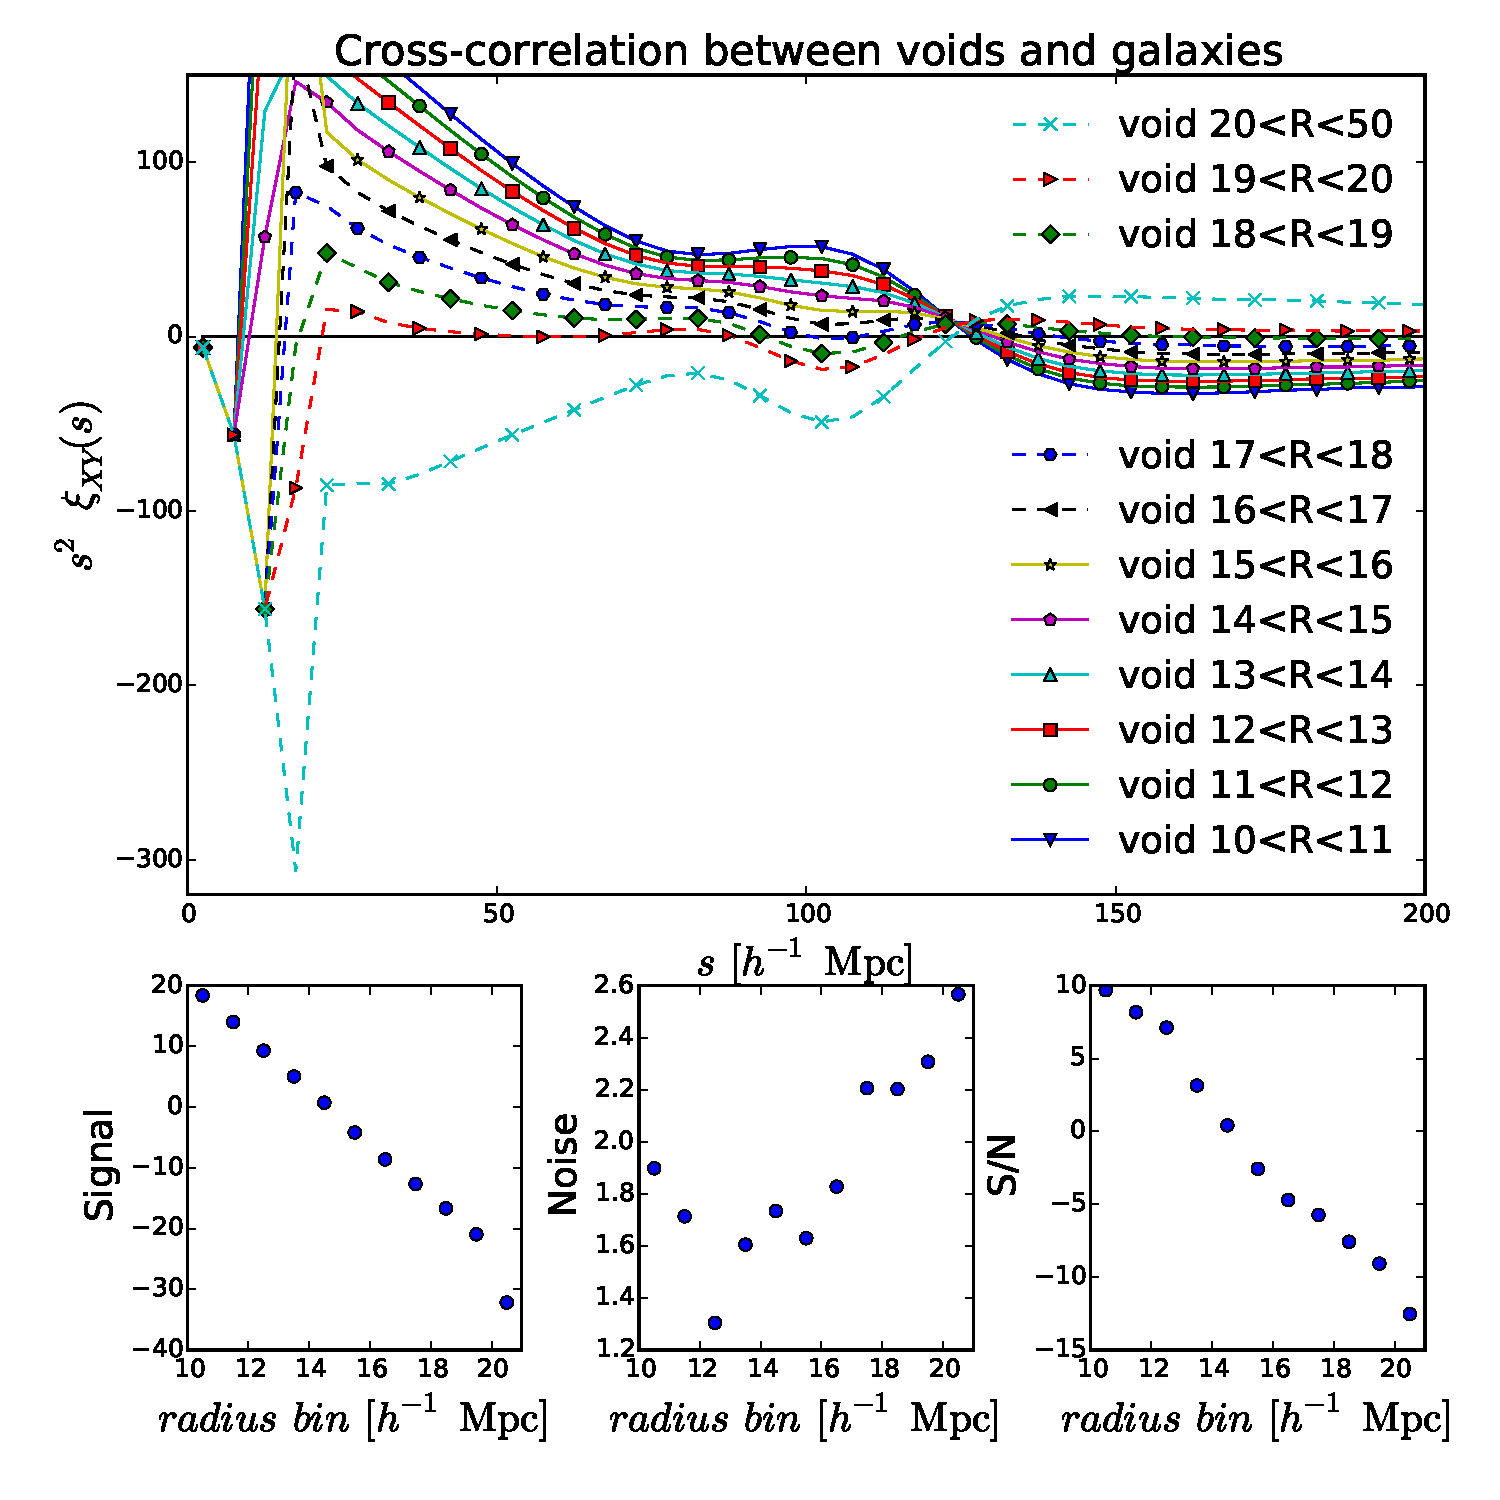
\includegraphics[width=.9\textwidth]{xcf_box_redshift_space_v_g_2016_01_29.pdf}
\caption{在红移$z = 0.56$处,100个红移空间完整模拟暗物质晕表通过DIVE得到的不同最小半径$R_1 < R < R_2$的巨洞与暗物质晕星的互相关函数(上图),和用第~\ref{sec:sn} 章测量BAO信号信噪比方法得到的$S$,$N$和$S/N$(下图)。(文献 ~\inlinecite{Liang2016}中的Figure 3)}
\label{fig:xcf_box_redshift_space_v_g}
\end{figure}

\begin{figure}
\centering
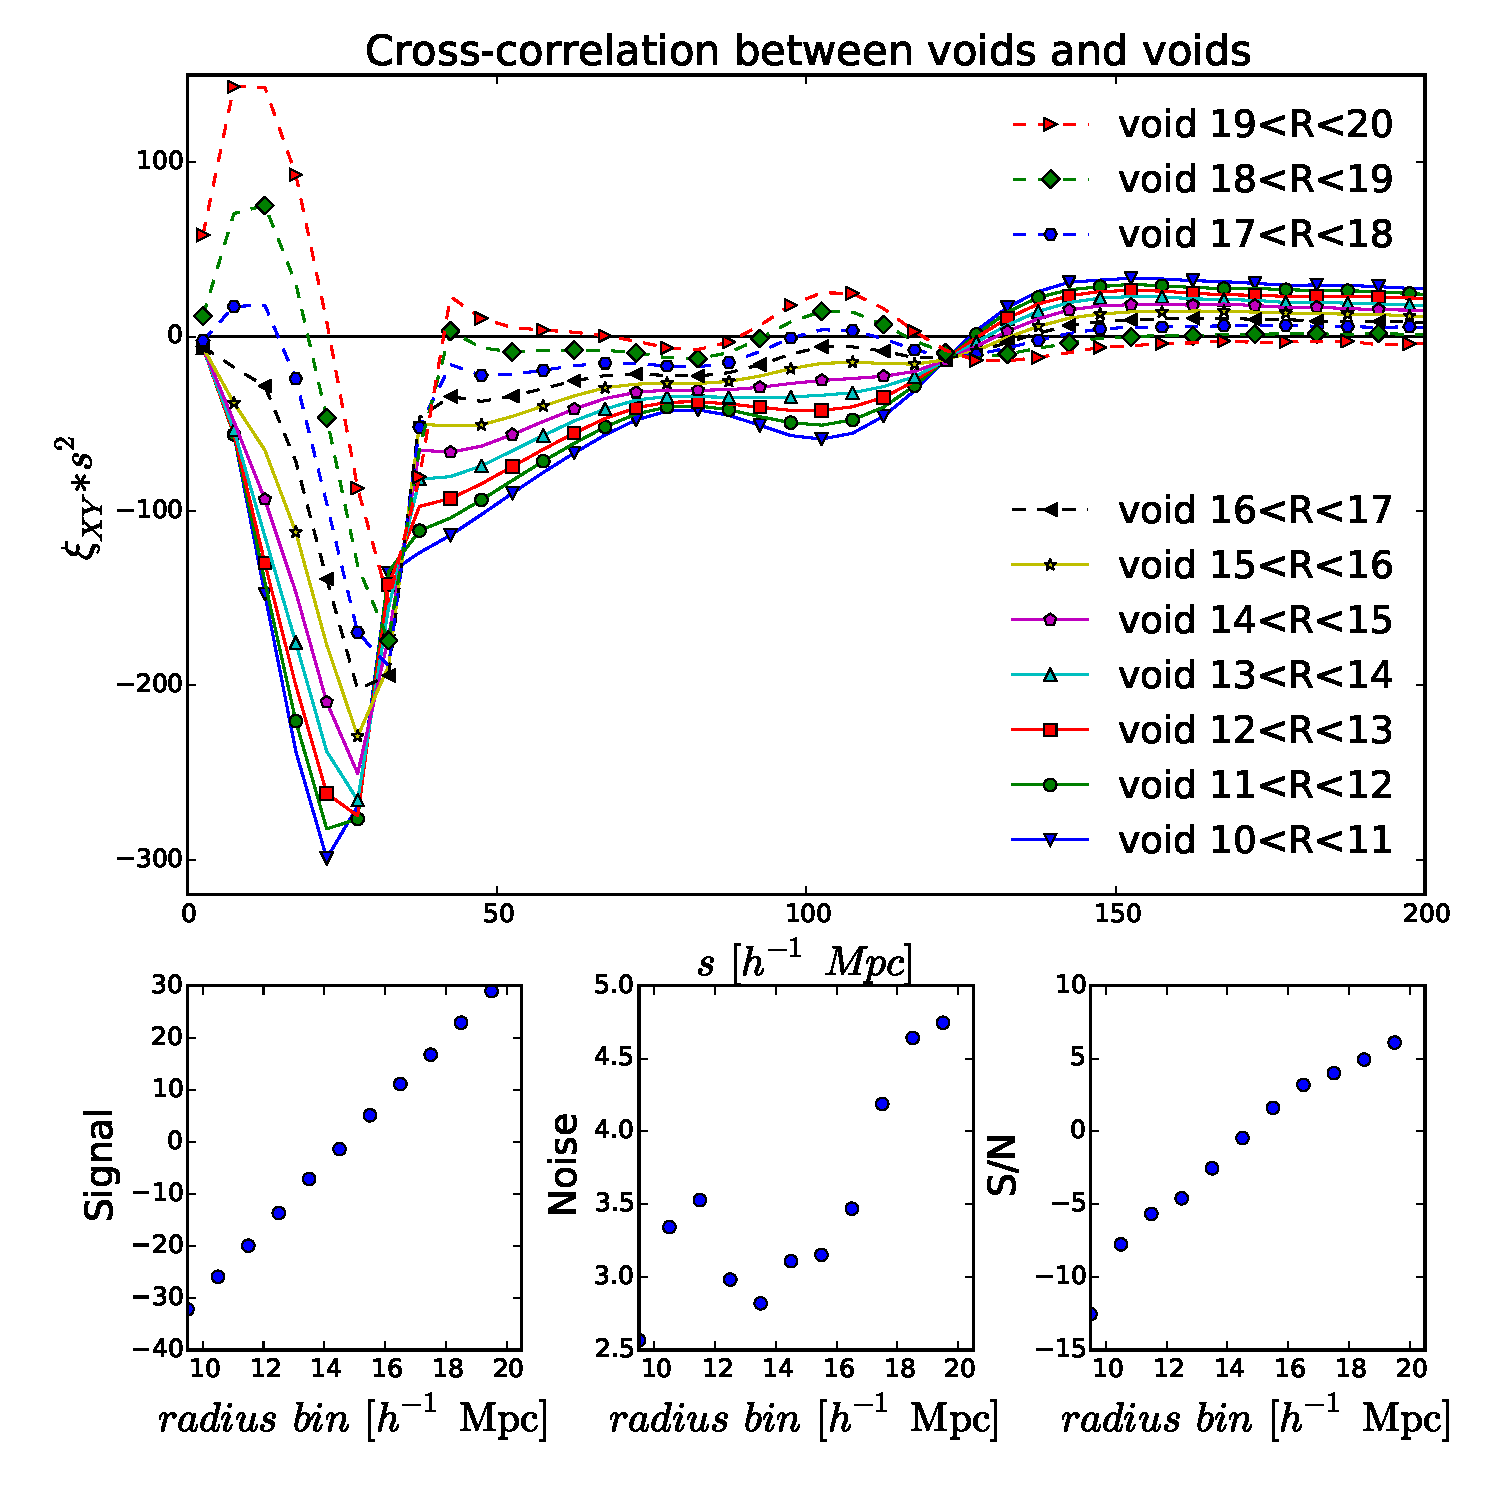
\includegraphics[width=.9\textwidth]{xcf_box_redshift_space_v_v_2016_01_29.pdf}
\caption{在红移$z = 0.56$处,100个红移空间完整模拟暗物质晕表通过DIVE得到的不同最小半径$R_1 < R < R_2$的巨洞与半径$20 < R < 50$ $h^{-1}$ Mpc的巨洞的互相关函数(上图),和用第~\ref{sec:sn} 章测量BAO信号信噪比方法得到的$S$,$N$和$S/N$(下图)。(文献 ~\inlinecite{Liang2016}中的Figure 3)}
\label{fig:xcf_box_redshift_space_v_v}
\end{figure}

为了进一步了解通过巨洞自相关函数的得到的BAO信号信噪比的特性,我们计算了红移空间内不同半径在 $R_1 < R < R_2$ 范围内巨洞子样本相对同一巨洞样本中半径$R_{\rm ref}>20$ $h^{-1}$ Mpc的巨洞子样本的互相关函数(图~\ref{fig:xcf_box_redshift_space_v_v}),和半径在 $R_1 < R < R_2$ 范围内巨洞子样本相对用来寻找巨洞的暗物质晕星的互相关函数(图~\ref{fig:xcf_box_redshift_space_v_g})。根据前文的研究结果我们可以确定半径$R_{\rm ref}>20$ $h^{-1}$ Mpc的巨洞子样本是真正宇宙学意义上的巨洞,即\textit{voids-in-voids}。它们的中心都在宇宙低密度区域,并且它们边界上的星系或暗物质晕的本动速度都朝向远离巨洞中心的方向~\cite{Zhao2016DIVE}。半径$R_{\rm ref}>20$ $h^{-1}$ Mpc的巨洞子样本和用来寻找巨洞的红移空间完整暗物质晕表是计算相关函数的参照样本(reference population)。

半径在 $R_1 < R < R_2$ 范围内巨洞子样本相对参照样本的互相关函数如果为正相关,则说明该巨洞子样本的中心所在的区域与参照样本在相同的宇宙大尺度环境,将相关函数如果为正的样本结合起来可以得到信噪比更高的BAO信号。例如,如果半径在 $R_1 < R < R_2$ 范围内巨洞子样本与半径$R_{\rm ref}>20$ $h^{-1}$ Mpc的巨洞子样本的互相关函数如果为正相关,那么将半径在 $R_1 < R < R_2$ 范围内巨洞子样本与半径$R_{\rm ref}>20$ $h^{-1}$ Mpc的巨洞子样本就都是\textit{voids-in-voids},将两个样本和在一起应该可以得到信噪比更高的BAO信号,反之的会得到信噪比更低的BAO信号。

然而图~\ref{fig:xcf_box_redshift_space_v_g} 和图~\ref{fig:xcf_box_redshift_space_v_v} 也展示了更为复杂的尺度依赖的偏袒(scale-dependent bias)。互相关函数的结果中,BAO特征尺度处的信号在$R \sim 15 h^{-1}$ Mpc附近改变方向,因为随着半径逐渐变小,DT巨洞逐渐从\textit{voids-in-voids}变为\textit{voids-in-clouds}。这也可以解释为什么图~\ref{fig:cf_box_r_bins_redshift_space} 中的$S/N$呈“V”字形而图~\ref{fig:cf_box_r_cuts_redshift_space} 的$S/N$呈反“V”字型,并且其拐点都在$R \sim 15 h^{-1}$附近。将半径$R \sim 15 h^{-1}$ Mpc的DT巨洞加入到半径$R > 15 h^{-1}$ Mpc的巨洞样本后,因为这两个样本的巨洞的中心在不同的环境中,所以和在一起计算2PCF时BAO信号就互相抵消了。

图~\ref{fig:xcf_box_redshift_space_v_g} 中在较大的距离时的互相关函数,即$s$ > 150 $h^{-1}$ Mpc的范围,展示了半径在 $R_1 < R < R_2$ 范围内巨洞子样本相对用来寻找巨洞的暗物质晕的线性偏袒$b_{vg}$。在$s \sim$ 150  $h^{-1}$ Mpc的距离以上,如果巨洞和暗物质晕的互相关函数为正,则$b_{vg}$为负。$19 < R < 20$和$20 < R < 50$ $h^{-1}$ Mpc这两个样本的互相关函数在大于$s \sim$ 150  $h^{-1}$ Mpc的距离为正,说明它们的$b_{vg}$为负。$18 < R < 19$ $h^{-1}$ Mpc的巨洞$b_{vg}$几乎为零。半径$R < 19$ $h^{-1}$ Mpc的巨洞$b_{vg}$为正,这一发现与之前其他研究的的结果一致~\cite{Hamaus:2013qja}。因为已知暗物质晕的线性偏袒$b_g$为正,所以较大巨洞($R > 19$ $h^{-1}$ Mpc)的线性偏袒$b_v$为负,较小巨洞$R < 19$ $h^{-1}$ Mpc的线性偏袒为正,半径$R \sim 19$ $h^{-1}$ Mpc的巨洞线性偏袒为零。而BAO特征尺度附近的信号在$R \sim 15$ $h^{-1}$ Mpc附近消失,这是巨洞和暗物质晕各自的非线性偏袒(the non-linear bias)造成的。因此巨洞的偏袒并不能简单的用其线性偏袒来表示,虽然半径$16 < R < 19$ $h^{-1}$ Mpc的巨洞的线性偏袒为正,但是它们的正BAO特征尺度附近的非线性偏袒为负,所以将这部分巨洞样本和半径$R \ge 19$ $h^{-1}$ Mpc的巨洞合起来可以得到信噪比最高的BAO信号,见图~\ref{fig:cf_box_r_cuts_redshift_space} 。

%In Fig.~\ref{fig:xcf}, all the cross-correlation functions intersect at one point around 130 $h^{-1}$ Mpc which is related to the size of the particle horizon at matter-radiation equality, estimated for the present Planck values \citep[][]{1994ApJ...428..399K,2011arXiv1111.2889P}. 
%%%%%Standard CDM cosmology fixes the size to be inversely proportional to the matter density $(h^2\,\Omega_{\rm M})^{-1}$, as discussed, e.g., by Peacock (1999). The linear correlation function crosses zero at this scale. Sylos Labini et al. (2009) have discussed to measure it for large scale galaxy surveys since the scale, $r_c$, is not sensitive to galaxy bias. 
%\citet[][]{2009A&A...505..981S} have discussed to measure the scale, $r_c$, where the galaxy correlation function turns from positive to negative.
%But, it is difficult to measure this scale due to the systematic errors and statistics uncertainty from observations. For voids clustering, the impact of observational systematics works differently so that one might observe $r_c$ in the void correlation function but not in the galaxy correlation function. However, we find that the uncertainty on the position of $r_c$ is large (see Fig.~\ref{fig:CFrealspace} and ~\ref{fig:CFzspace}). 
%because of the non-linear bias previously discussed. Thus, it would be even more difficult to extract reliable cosmological information from the measurement of $r_c$ from the void correlation function.

\subsection{用不含BAO的实空间完整模拟暗物质晕表研究巨洞BAO信号}
\label{sec:wigglenonwiggle}
\begin{figure}
\centering
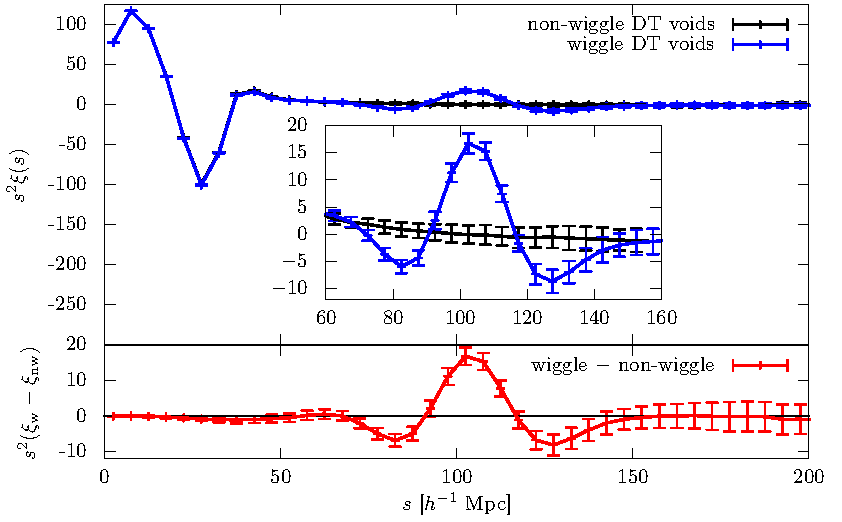
\includegraphics[width=.9\textwidth]{simd}
\caption{ 在红移$z = 0.56$处,100个实空间完整模拟暗物质晕表中通过DIVE得到的半径$R \geq 16$ $h^{-1}$ Mpc的巨洞的平均2PCF和标准差。上半部分中,蓝色实线和蓝色误差棒表示初始密度场有BAO的实空间完整模拟暗物质晕表的巨洞结果(wiggle DT voids),黑色实线和黑色误差棒表示初始密度场没有BAO的实空间完整模拟暗物质晕表的巨洞结果(non-wiggle DT voids)。下半部分的红色实线与红色误差棒表示两组实空间完整模拟暗物质晕表巨洞2PCF的残差(wiggle - non-wiggle)的均值和标准差,黑色实线标记了图中取值为0的位置。(文献 ~\inlinecite{Kitaura2016Void} 中的FIG. 1)}
\label{fig:wigglenonwiggle}
\end{figure}

第~\ref{sec:datanw} 章介绍了不含BAO的实空间完整模拟暗物质晕表,使用DIVE可以得到其中的巨洞数据,计算其中半径$R \geq 16$ $h^{-1}$ Mpc的巨洞2PCF(non-wiggle DT voids)。用第~\ref{sec:completeoptr} 章得到的实空间完整模拟暗物质晕表的最佳巨洞子样本的2PCF(wiggle DT voids)减去non-wiggle DT voids的2PCF,得到的就是纯粹的BAO信号。wiggle DT voids与non-wiggle DT voids的区别只是他们的初始密度场一个有BAO另一个没有BAO,最终体现在两组数据中巨洞2PCF的差异只是原初密度场中BAO信号造成的影响。wiggle DT voids与non-wiggle DT voids的2PCF都在小距离处存在一些与最小半径相关的振荡特征,这是由巨洞排斥效应造成的,图~\ref{fig:wigglenonwiggle} 的结果表明在$s \sim 100$ $h^{-1}$ Mpc处的信号是真实的BAO信号,而不是巨洞排斥效应在较大距离处的特征信号。另外,图~\ref{fig:wigglenonwiggle} 也清晰的展示了第~\ref{sec:sn} 章里提到的在巨洞BAO特征尺度的左右两边存在两个明显的低谷,我们利用这两个低谷和BAO特征尺度处的信号定义了不依赖具体模型的估计BAO信号显著性的方法。

\subsection{实空间完整模拟暗物质晕表内不重叠的巨洞样本}
\label{sec:disjoint}
\begin{figure}
\centering
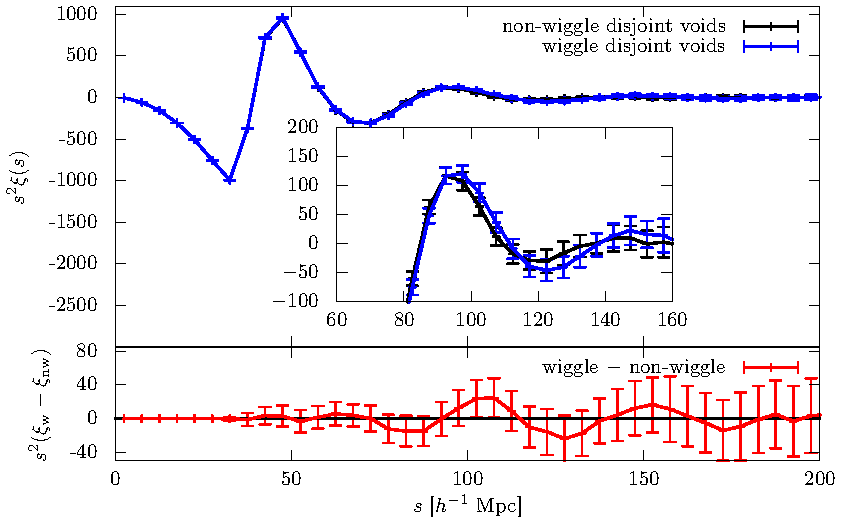
\includegraphics[width=.9\textwidth]{nosimd}
\caption{与图~\ref{fig:wigglenonwiggle}一样的研究方法用于不重叠的巨洞样本。此时虽然在$s \sim 100$ $h^{-1}$ Mpc处也存在信号,但是其误差与信号具有相同的强度,而且在$s \sim 150$ $h^{-1}$ Mpc处也存在类似的特征。(文献 ~\inlinecite{Kitaura2016Void} 中的FIG. 2)}
\label{fig:disjoint} 
\end{figure}

用第~\ref{sec:datacomple} 章和第~\ref{sec:datanw} 章介绍的数据通过DIVE获得的巨洞被称为DT巨洞,其特点是我们允许不同的巨洞之间互相重叠。而以前人们定义巨洞的方式并不允许巨洞之间互相重叠。在本节我们模仿之前人们对巨洞的定义,在DT巨洞样本之内找到互相不重叠的最大的巨洞子样本,被称为不重叠的巨洞样本(disjoint voids),具体方法可以参考HB void finder~\cite{Patiri2006372}。

利用第~\ref{sec:wigglenonwiggle}的方法,同样可以计算wiggle disjoint voids与non-wiggle disjoint voids得到disjoint voids的BAO信号,结果请见图~\ref{fig:disjoint} 。disjoint voids互相之间不重叠,因此其数密度相比同样大小的DT voids低很多,其巨洞排斥效应更强,从而无法探测到到可靠的BAO信号。这可能就是为什么之前的工作中虽然研究过巨洞的2PCF,但从来没有人试图用巨洞探测BAO特征尺度的原因。

巨洞分布在宇宙的低密度区域,原初宇宙中的低密度区域随着演化会逐渐连成一片,使得在晚期很难观测到低密度区域的子结构。而通过允许重叠,DT巨洞一方面不依赖具体宇宙学模型即可近似得到低密度区域的子结构信息,另一方面也大大降低了DT巨洞在大尺度上的巨洞排斥效应,从而使得重子声波振荡信号可以从DT巨洞的成团性分析中得到。

\section{用模拟光锥星系表研究巨洞的BAO信号}

在这一节,我们将会使用模拟光锥星系表来研究其中巨洞的BAO信号。相对完整模拟暗物质晕表,模拟光锥星系表在很多性质上跟真实的观测数据是完全一样的,比如它们在天球上的分布,数密度随红移的变化,以及因观测条件限制造成的选择效应等,在第~\ref{sec:lightcone} 章详细介绍了模拟光锥星系表。这一节的工作都是基于BOSS/SDSS-III CMASS DR11的\textsc{patchy}模拟光锥星系表完成的,这一节都简称为\textsc{patchy}模拟光锥星系表。我们一共使用了1024个模拟光锥星系表,它是专门为BOSS/SDSS-III CMASS DR11的观测数据而生成的,同时也是BOSS/SDSS-III CMASS DR11官方发布公开的数据。第~\ref{sec:lcdata} 章介绍了如何使用DIVE在模拟光锥星系表中寻找巨洞,第~\ref{sec:lc2pcf} 章阐述了如何估算模拟光锥星系表的2PCF及如何构建随机样本用以估算模拟光锥星系表的2PCF,最后第~\ref{sec:lcoptr} 章分析了模拟光锥星系表的巨洞BAO信号。

\subsection{构建模拟光锥星系表的巨洞数据}
\label{sec:lcdata}

\begin{figure}
\centering
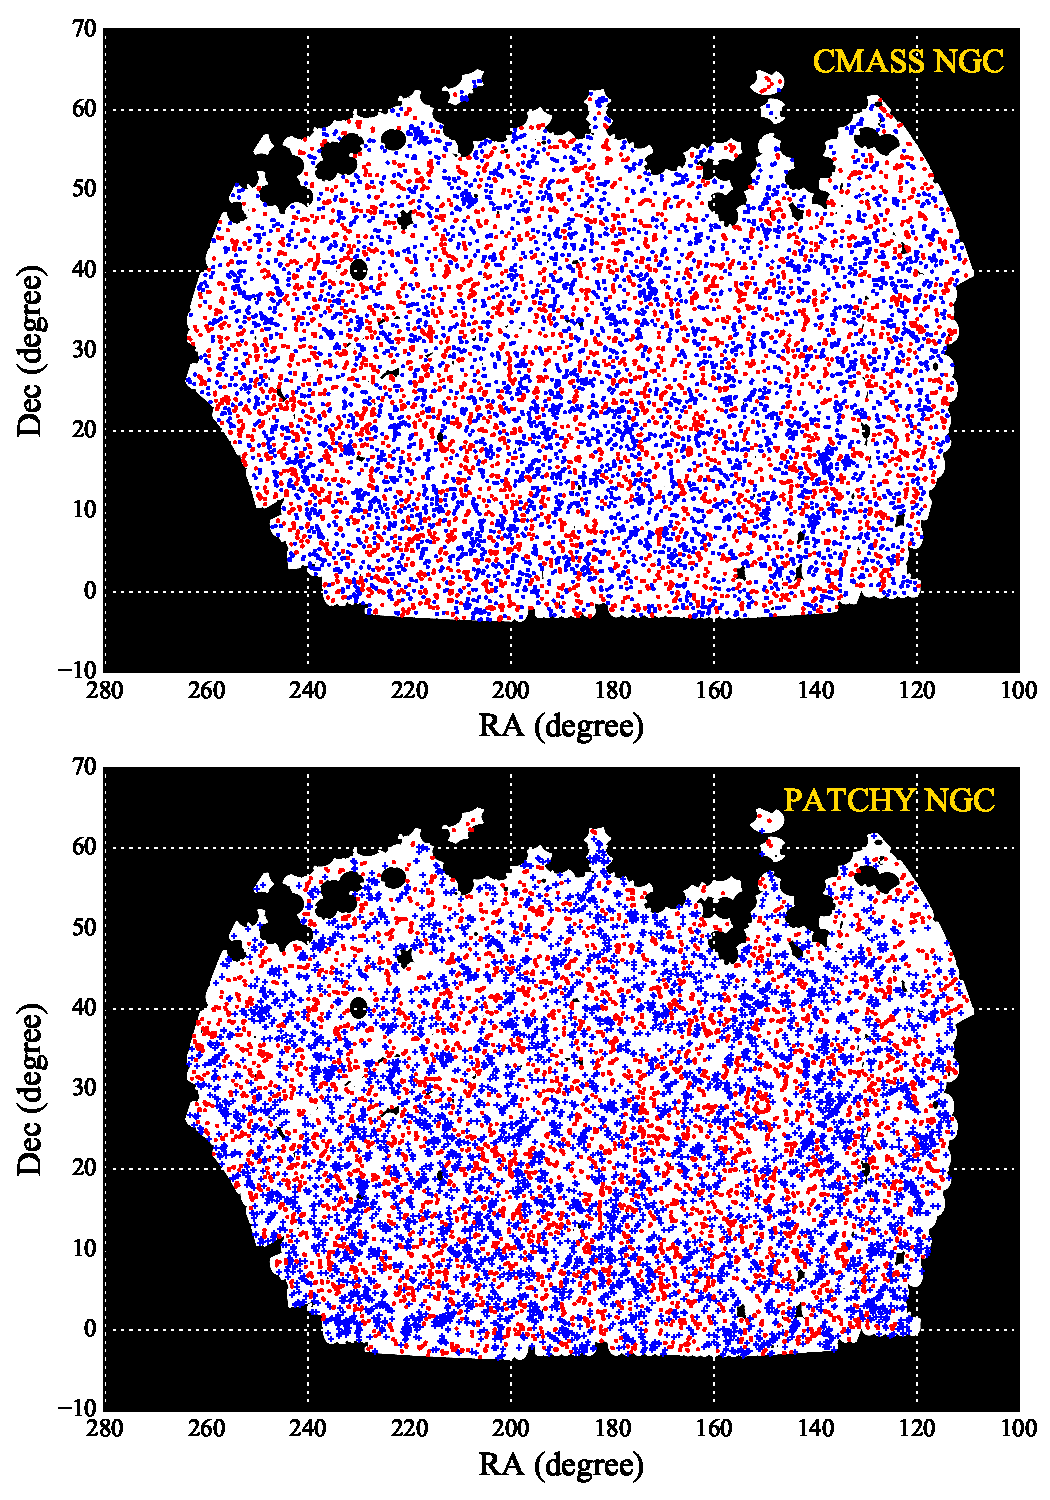
\includegraphics[width=.9\textwidth]{dr11_mock}
\caption{红移$0.498 < z < 0.5$区间内,\textsc{MultiDark PATCHY} BOSS NGC CMASS DR11的观测数据(上图,“CMASS NGC”)和模拟光锥星系表(下图,“\textsc{PATCHY} NGC”)中星系(蓝色{\color{blue} +})和半径$R > 16$ $h^{-1}$ Mpc的巨洞中心位置在天球坐标(RA,DEC)上的投影。黑色区域是巡天中不能被有效观测的区域。(文献 ~\inlinecite{Liang2016}中的Figure 4)}
\label{fig:cmass_sky_ngc}
\end{figure}

为了使模拟光锥星系表和真实的观测数据保持一致,其记录的位置信息是两个球面坐标和红移(RA,DEC,z)。所以使用DIVE寻找巨洞前后需要一些额外的步骤进行坐标转换和其他处理,具体步骤如下:
%To obtain the void catalogues from the input lightcone galaxy catalogues we present now a series of  steps which takes care of the survey geometry and selection function:
\begin{description}
%\item[1.]filter the galaxy mocks with the veto flag and fiber collision flag.
\item[1.] 将天球坐标(RA,DEC)和红移z转换成共动距离下的笛卡尔坐标($x_1$,$x_2$,$x_3$),这一步需要假设一个基准宇宙学模型来将红移转换成共动距离。
\item[2.] 使用DIVE在共动距离下笛卡尔坐标系的模拟光锥星系表里寻找巨洞。
\item[3.] 将所有巨洞的中心坐标从共动距离下的笛卡尔坐标系($x_1$,$x_2$,$x_3$)转换成球面坐标加红移(RA,DEC,z),这时还会用到第一步假设的基准宇宙学模型。
\item[4.] 因为各种观测条件限制,真正可以被有效观测的星系只分布在天球的一部分区域。所以如果巨洞的中心不在有效观测区域内的话就会被从样本中移除。这一步我们使用了文献 ~\inlinecite{2014MNRAS.437.2594W}中介绍的方法和代码\footnote{\url{https://github.com/mockFactory/make_survey}}。
\end{description}

尽管模拟光锥星系表的星系都在巡天的有效观测区域内,但是使用DIVE得到的巨洞的中心可能会在有效观测区域以外。所以为了得到可靠的巨洞数据,必须将中心不在有效观测区域的巨洞移出样本。我们定义的巨洞是一个空心球,所以如果巨洞的一部分体积在有效观测区域之外就将其移除的话可以得到一个更加合理的巨洞样本。为了实现这个目的,可以在有效区域的边界随机生成很多点,如果巨洞中存在这些随机生成的点就说明巨洞的一部分体积在有效区域之外而应该被从样本中移除。但是,我们发现这样做的结果对研究巨洞的BAO信号并没有什么实质性的影响,但却会大大增加计算量,因此我们最终只将中心在有效区域外的巨洞从样本中移除。图~\ref{fig:cmass_sky_ngc}展示了半径$R \geq 16\,h^{-1}$Mpc的DT巨洞中心和星系在(RA,DEC)平面上的投影,DT巨洞的中心都分布在有效观测天区内没有星系的空旷区域里。

因为巨洞的中心和半径是由四个星系组成的空心四面体决定的,如果其中一个星系因为在有效观测区域之外而没被观测到,那么就将无法通过DIVE找到这个本该存在的巨洞。而如果有效区域之外存在一个未被观测到的星系,那么这个未被观测到的星系和它附近在有效区域内的其他星系可能会构成一些新的空心四面体,这个星系也可能存在于通过有效区域内的星系而找到的巨洞内部。因不能确定模拟光锥星系表和真实观测数据的边界之外的星系的位置而造成通过DIVE找到的边界上的巨洞与真实的巨洞存在的偏差被称为边界效应。边界效应会改变在边界附近巨洞的数密度从而影响到巨洞成团性的研究结果,在后文中将介绍如何巧妙的通过生成具有同样边界效应的随机样本来降低边界效应对成团性研究结果的影响。

根据第~\ref{sec:voidnumberdensity} 章的结果可知,在完整模拟暗物质晕表内巨洞的半径不可能大于50 $h^{-1}$ Mpc,但是在模拟光锥星系表内存在一些半径大于50 $h^{-1}$ Mpc的巨洞。这主要是由边界效应造成的,所以我们最终计算巨洞的2PCF时,只使用了半径小于50 $h^{-1}$ Mpc的巨洞。半径大于50 $h^{-1}$ Mpc的巨洞在整个巨洞样本中的比例非常小,移除这部分数据对整体的统计性不会造成影响。

\subsection{测量模拟光锥星系表巨洞数据的2PCF}
\label{sec:lc2pcf}
\subsubsection{用于估计模拟光锥星系表巨洞数据2PCF的方法}
\label{sec:lclzest}

在第~\ref{sec:baorecon} 章提到有很多种估算2PCF的方法,但因The Landy \& Szalay estimator较其他方法更为准确从而被广泛应用。所以我们也使用了公式~(\ref{EQ:lsestimator})来计算模拟光锥星系表的2PCF。和完整模拟暗物质晕表不同的是,这时无法通过一个解析的公式准确计算公式~(\ref{EQ:lsestimator})的$DR$和$RR$项。所以除了需要计算其2PCF的样本数据之外还需要一个随机样本。

为了BOSS/SDSS-III CMASS DR11所公布的数据中包括用于计算星系2PCF所需要的随机样本,在此被称为星系随机样本。但是因为不同半径的巨洞在观测区域内不同位置的分布可能会有很大区别,而星系在整个区域内的分布较为平均,所以不能直接简单的使用星系随机样本来计算巨洞的2PCF。我们需要为巨洞单独制作一份随机样本来计算其2PCF。

\subsubsection{构建模拟光锥星系表巨洞数据2PCF的随机样本}
\label{sec:lcrandom}

接下来介绍如何生成一个随机样本使其在RA、DEC和红移三个方向都有与巨洞一样的数密度分布。用这样的随机样本计算巨洞的2PCF可以有效的去除边界效应和巡天有效区域不规则的几何形状等问题的影响,因此这个随机样本被称为巨洞随机样本。

在此我们使用了一种类似洗牌的方式~\cite{Anderson2014441}来获取巨洞随机样本并保证其在RA、DEC和红移三个方向都有与巨洞一样的数密度分布。巨洞数据包括坐标和半径,可以分为两部分:球面坐标(RA,DEC)和红移及半径(z,R)。为了保证数密度随红移的分布保持不变,需要从数据中获得红移及半径(z,R)。然后在有效观测的天球区域内生成(RA,DEC)并把随机生成的(RA,DEC)与从数据获得(z,R)结合起来就可以得到随机样本,这也是BOSS/SDSS-III项目中生成星系随机样本的方式。然而因为巨洞具有边界效应,这种方法不适用于生成巨洞随机样本。

\begin{figure}
\centering
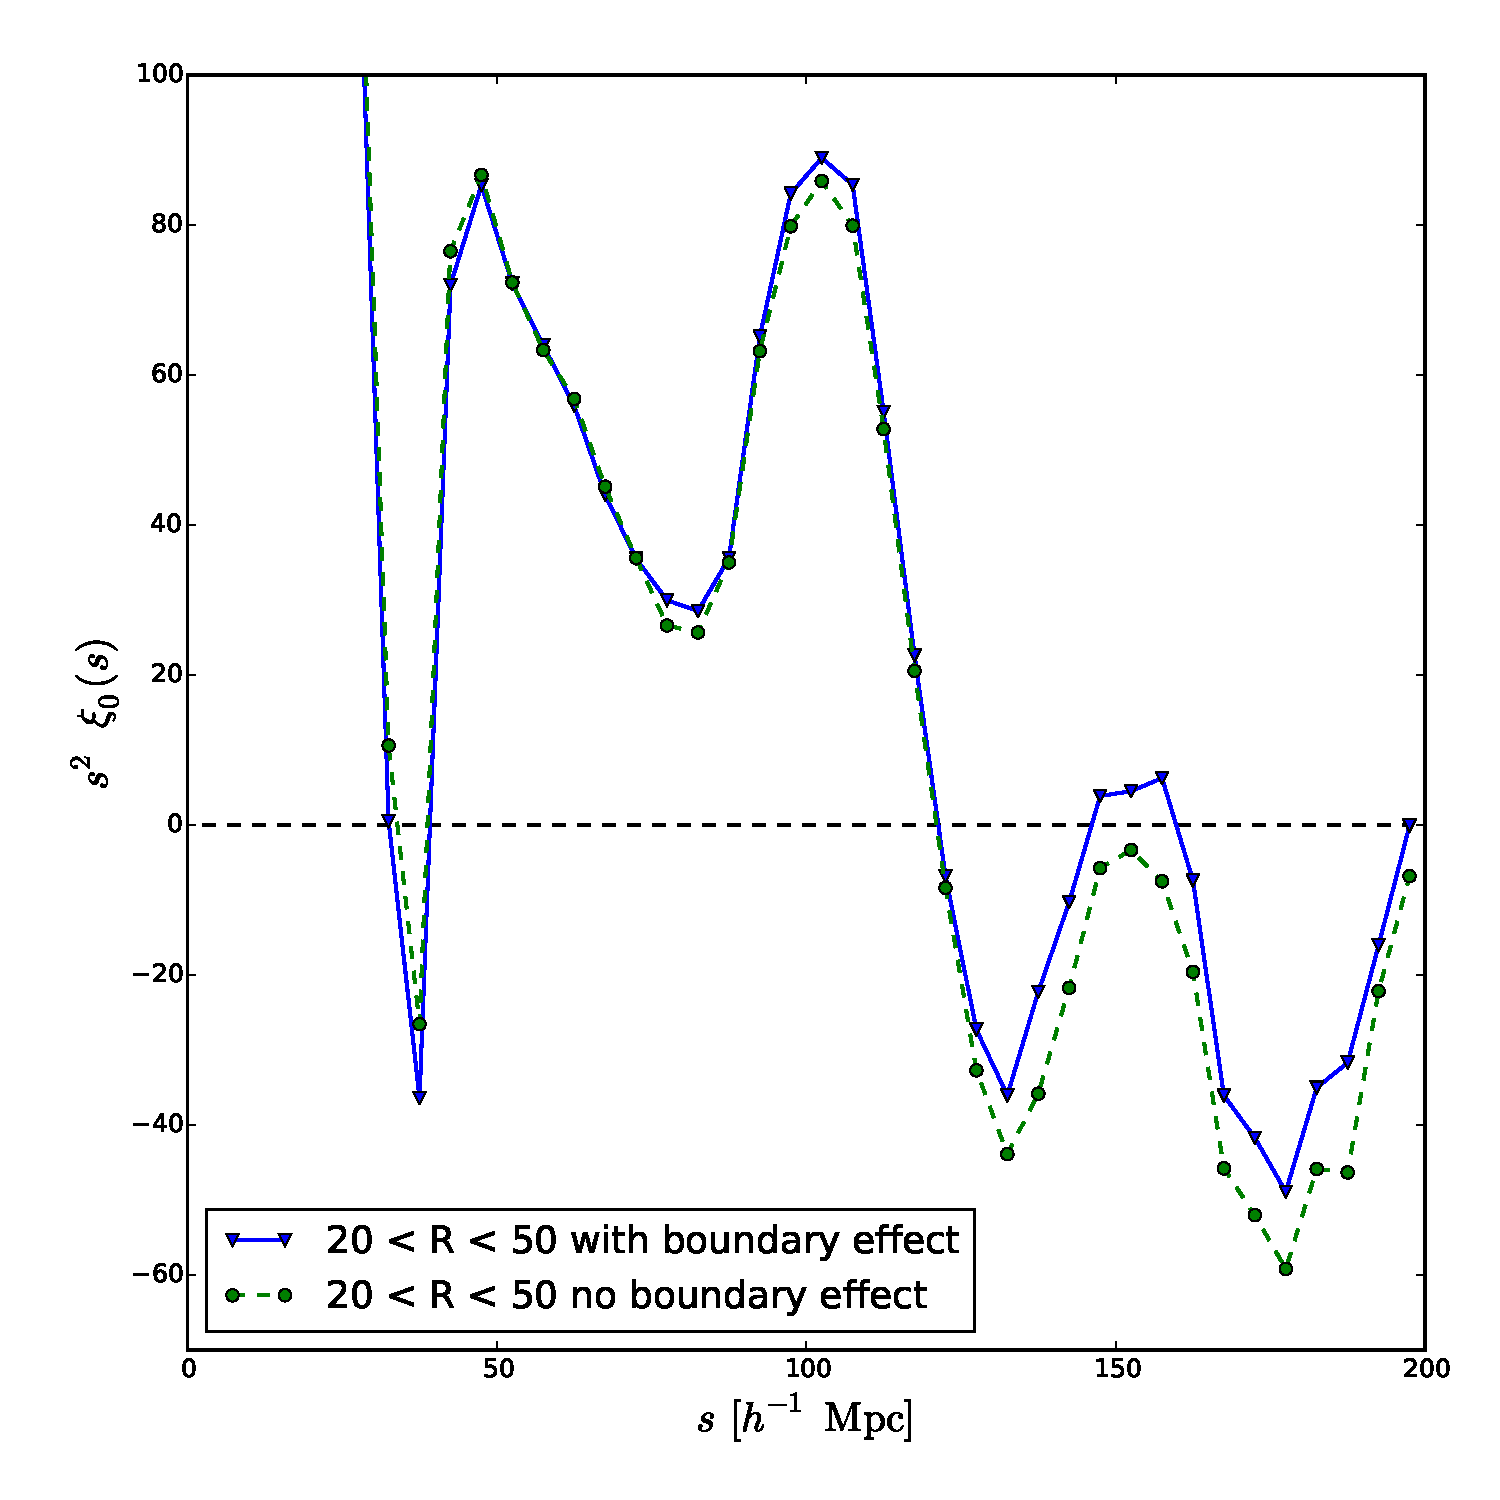
\includegraphics[width=.9\textwidth]{cf_boundary_2015_11_13.pdf}
\caption{有边界效应的巨洞2PCF(蓝色实线)对比没有边界效应的巨洞2PCF(绿色虚线)。(文献 ~\inlinecite{Liang2016}中的Figure 5)}
\label{fig:cf_boundary}
\end{figure}

在介绍如何生成巨洞随机样本之前,我们先通过一个实验来说明边界效应对巨洞成团性研究结果的影响。将完整的实空间模拟暗物质晕表从笛卡尔坐标系转换成球面坐标加红移,选取在$10<{\rm RA}<80$、$10<{\rm DEC}<50$和$0.4<z<0.7$为巡天观测的有效区域。这些暗物质晕在每个方向上都是均匀分布,所以其随机样本也应该是均匀随机分布的。
\begin{itemize}
\item 实验组数据, 实验组数据以如下方式受到了边界效应影响:先将有效区域外的暗物质晕移除,然后按第~\ref{sec:lcdata} 章介绍的方法用DIVE寻找巨洞。
\item 对照组数据, 对照组数据没有受到边界效应影响,因为我们按第~\ref{sec:lcdata} 章介绍的方法用DIVE寻找巨洞之前没有将有效区域之外的暗物质晕移除。
\end{itemize}
也就是说,对照组数据等效于用实空间完整模拟暗物质晕表寻找巨洞,而实验组数据缺失了在有效观测区域之外暗物质晕从而在边界产生了边界效应。用实验组数据的巨洞计算2PCF其结果应该与第~\ref{sec:voidbaocomplete} 章的结果相同。因为实验组与对照组最终的有效区域相同,所以这两数据应该收到同样宇宙方差(cosmic variance)的影响。我们一共使用了20个实空间模拟暗物质晕表来生成这两组数据。图~\ref{fig:cf_boundary} 中展示了边界效应造成相关函数在较大的距离处相对真实值变大了一点,但是BAO特征尺度的位置和2PCF的整体形状几乎没有任何变化。因为两条曲线的误差几乎一样,图中没有标注误差棒的大小。

模拟光锥星系表和观测数据有同样的有效观测区域和边界效应,我们把100个光锥中的巨洞数据合并起来,合并起来的数据与模拟光锥星系表的巨洞数据有同样的数密度分布和边界效应。需要注意的是,在不同红移处巨洞的数密度分布会不完全一样,所以其边界效应也不尽相同。因此我们从合并的数据中获取随机的球面坐标(RA,DEC)和红移与半径(z,R),然后通过随机洗牌的方式将(RA,DEC)和(z,R)重新组合成为巨洞随机样本,具体步骤如下:
\begin{description}
\item[1.] 将100个光锥中的巨洞数据合并起来得到合并数据。
\item[2.] 将合并数据按照红移分为$0.45 < z < 0.55$和$0.55 < z < 0.65$两组。
\item[3.] 将上面的两组数据再按半径不同分为如下五组,$16<R<17$、$17<R<18$、$18<R<19$、$19<R<20$、$20<R<50$ $h^{-1}$ Mpc。现在合并数据一共被分为10组。
\item[4.] 将每组数据分为球面坐标(RA,DEC)和红移与半径(z,R)两部分,然后再随机洗牌将这两部分组合起来。
\item[5.] 将随机洗牌后的10组数据合并成一组数据。
\end{description}

\begin{figure}
\centering
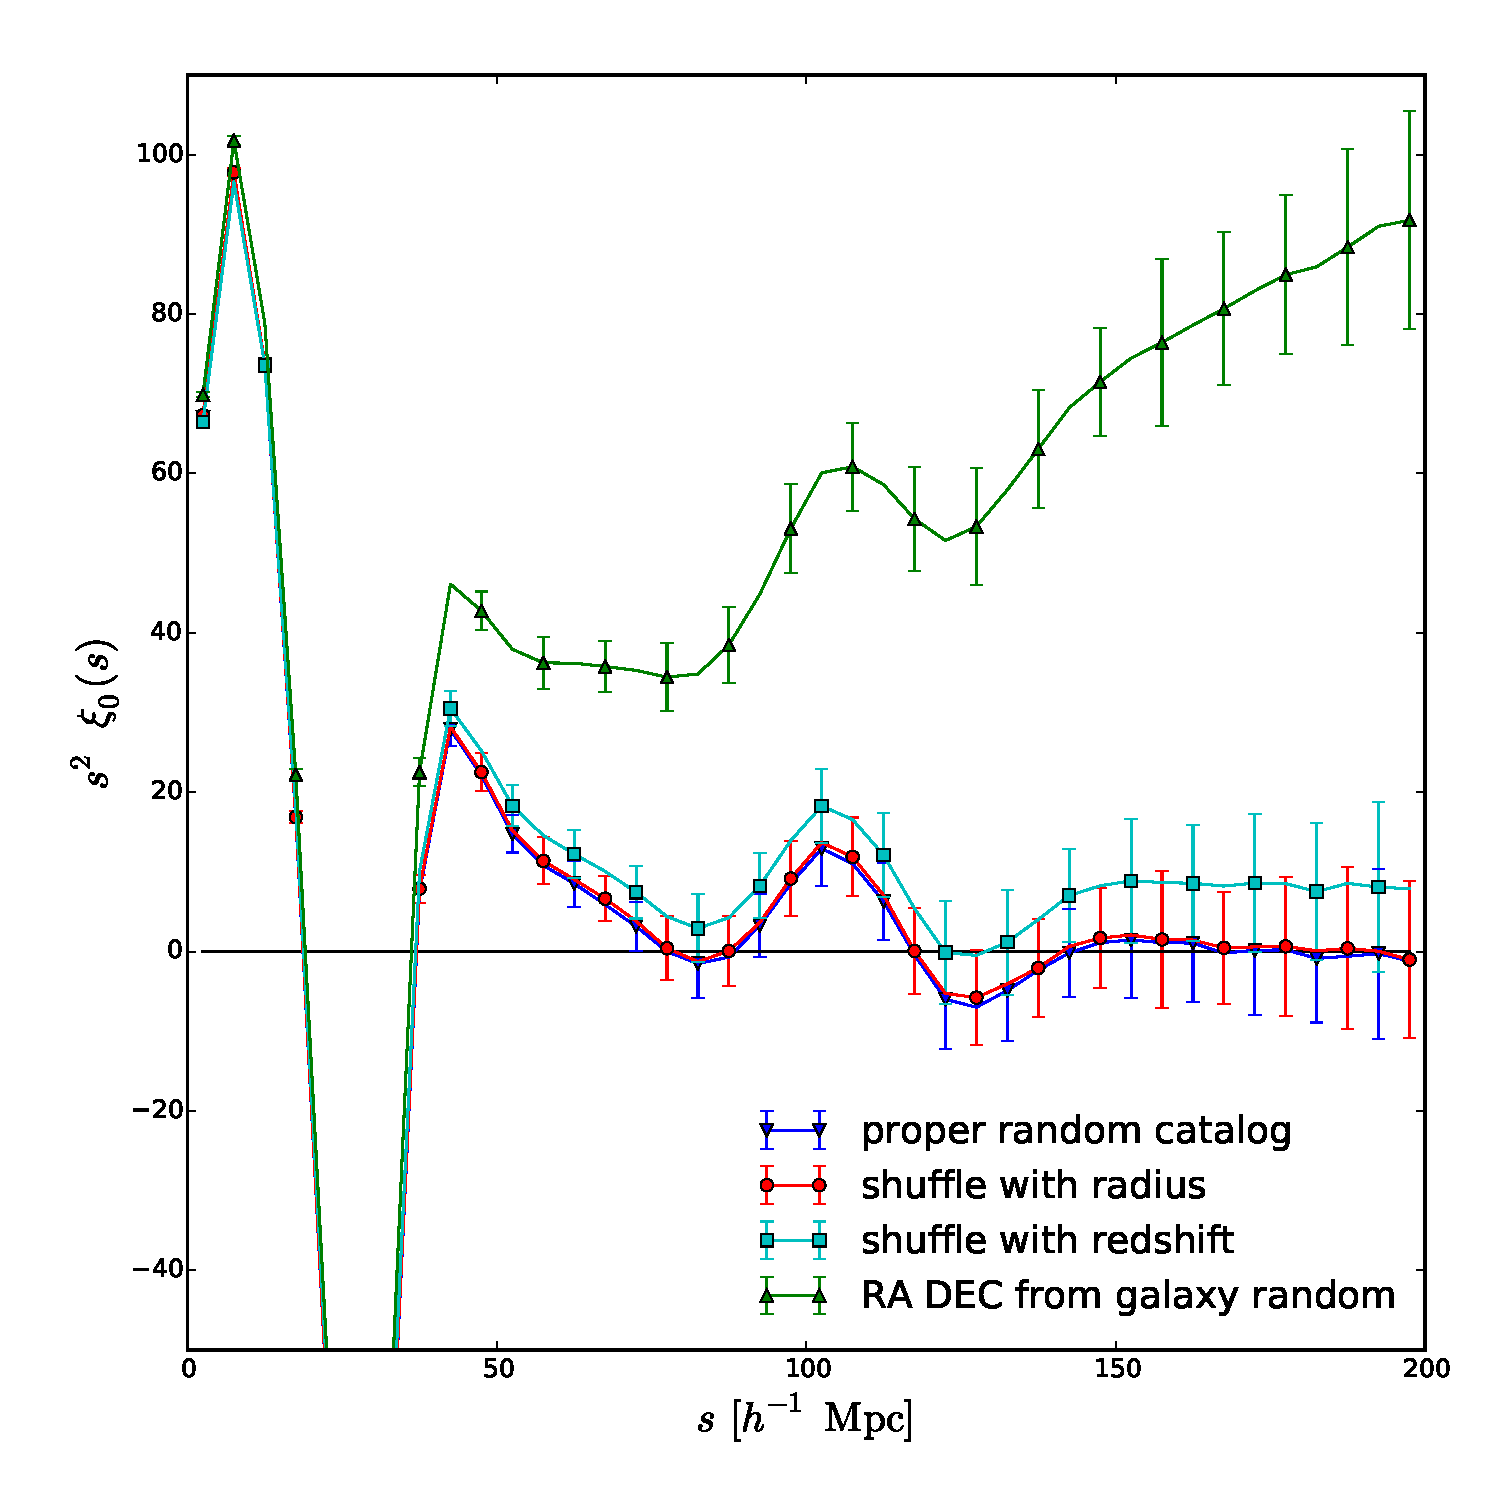
\includegraphics[width=.9\textwidth]{cf_lightcone_N_shuf_test_2015_11_13.pdf}
\caption{同一组巨洞样本用不同随机样本计算得到的2PCF:蓝色实线是用适当的随机样本计算的结果,青色实线是通过缺省第3步(没有分不同半径进行随机洗牌)的随机样本得到的2PCF,红色实线是通过缺省第2步(没有分不同红移进行随机洗牌)的随机样本得到的2PCF,绿色实线是使用星系随机样本计算得到的2PCF。(文献 ~\inlinecite{Liang2016}中的Figure 6)}
\label{fig:cf_lightcone_N_shuf_test}
\end{figure}

图~\ref{fig:cf_lightcone_N_shuf_test} 展示了用随机洗牌的方式生成的随机样本所计算的巨洞2PCF,及用其他几种方式成的随机样本计算的巨洞2PCF,如使用随机洗牌但是省略第二部或第三步的结果。使用星系随机样本计算巨洞2PCF的结果也在图中~\ref{fig:cf_lightcone_N_shuf_test} 中。从结果的对比可以发现,省略第三步会使2PCF的计算结果偏大,而使用星系随机样本会使结果严重偏离正常值。因为合并样本被分成球面坐标(RA,DEC)和红移与半径(z,R)两部分,红移与半径之间的关系被保持下来,所以省略第二步对结果的影响较小。边界效应在一定程度上造成用不恰当的随机样本计算的巨洞2PCF相对正确结果偏大,而使用星系随机样本会放大边界效应造成结果严重偏离正确值。

因此,使用这一节介绍的方法生成巨洞随机样本对于准确估算巨洞的2PCF非常重要,这也是本工作相较用星系成团性探测BAO信号的突出创新点和难点。

\subsection{模拟光锥星系表内测量巨洞BAO信号的最佳子样本}
\label{sec:lcoptr}

\begin{figure}
\centering
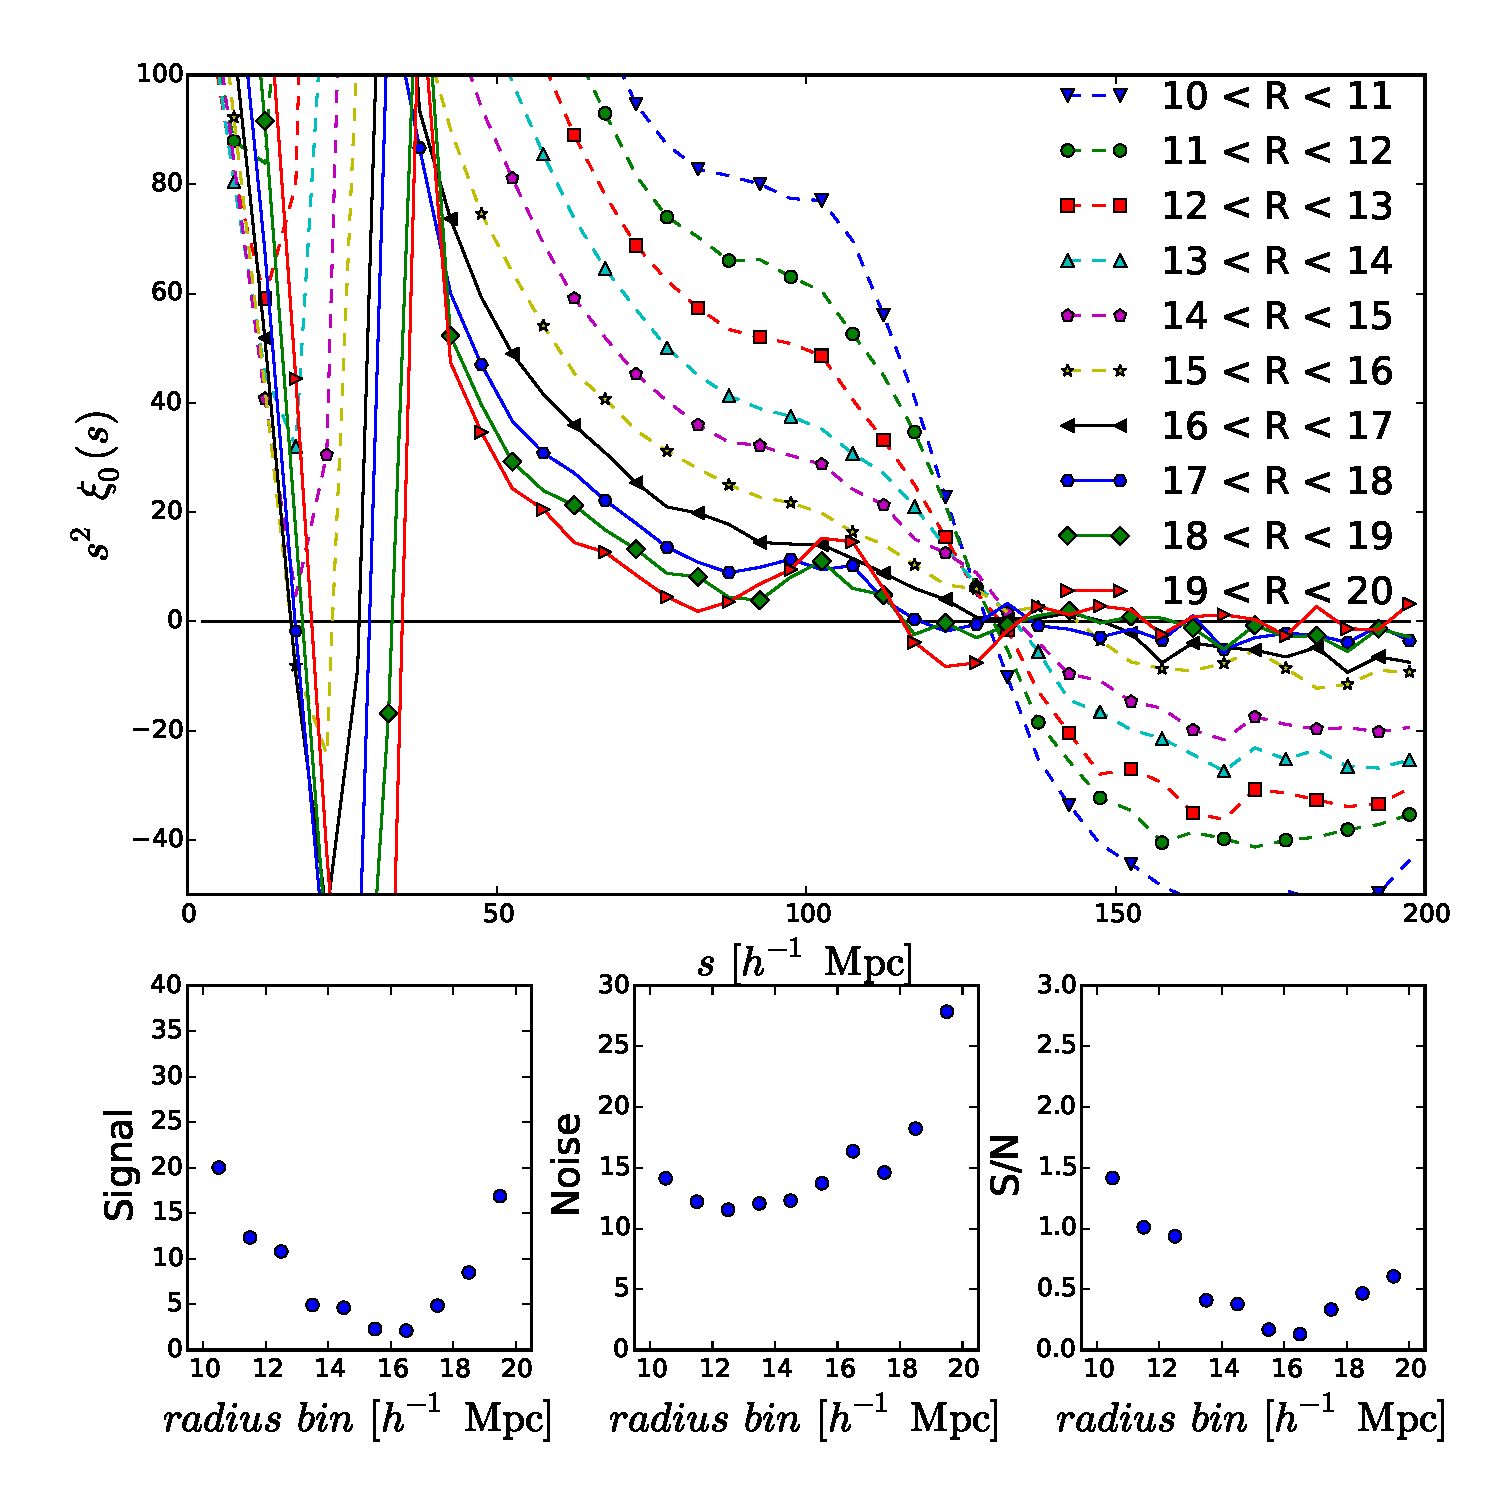
\includegraphics[width=.9\textwidth]{cf_lightcone_r_bins_2015_11_13.pdf}
\caption{前100个BOSS CMASS NGC DR11样本的\textsc{PATCHY}模拟光锥星系表的巨洞数据在不同半径区间 $R_1 < R < R_2$的平均2PCF,和用第~\ref{sec:sn} 章测量BAO信号信噪比方法得到的$S$,$N$和$S/N$。(文献 ~\inlinecite{Liang2016}中的Figure 7)}
\label{fig:cf_lightcone_r_bins}
\end{figure}

\begin{figure}
\centering
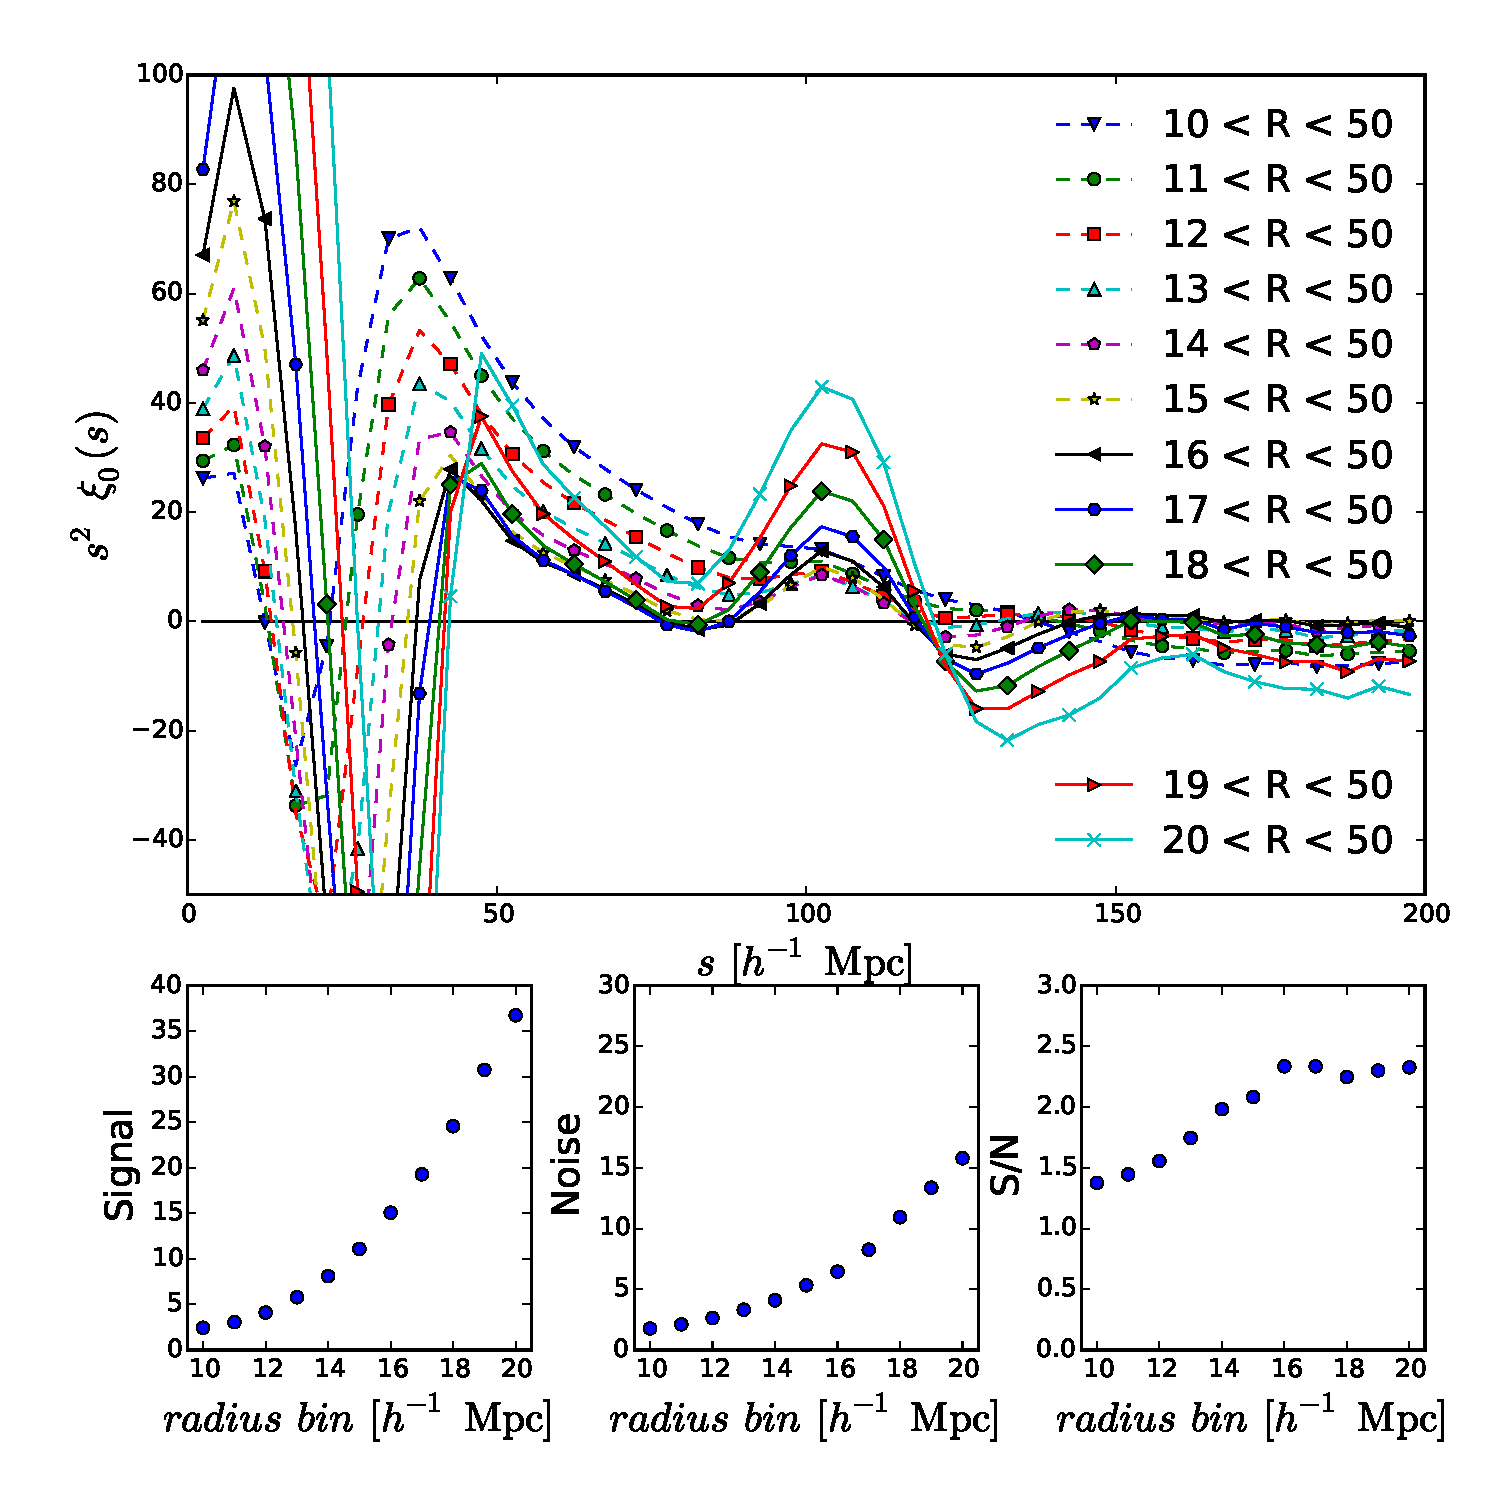
\includegraphics[width=.9\textwidth]{cf_lightcone_r_cuts_2015_11_13.pdf}
\caption{前100个BOSS CMASS NGC DR11样本的\textsc{PATCHY}模拟光锥星系表的巨洞数据在不同最小半径处 $R>R_{\rm cut}$的平均2PCF,和用第~\ref{sec:sn} 章测量BAO信号信噪比方法得到的$S$,$N$和$S/N$。(文献 ~\inlinecite{Liang2016}中的Figure 7)}
\label{fig:cf_lightcone_r_cuts}
\end{figure}

使用第~\ref{sec:lcrandom} 章生成的巨洞随机样本,我们计算了前100个BOSS/SDSS-III CMASS-NGC模拟光锥星系表的巨洞2PCF。2PCF的结果和使用第~\ref{sec:sn} 章测量BAO信号信噪比方法得到的$S$,$N$和$S/N$请见图~\ref{fig:cf_lightcone_r_bins} 和图~\ref{fig:cf_lightcone_r_cuts} 。

图~\ref{fig:cf_lightcone_r_bins}和图~\ref{fig:cf_lightcone_r_cuts} 中的$S/N$相比完整模拟暗物质晕表的结果偏低,这与我们的预期一致,因为模拟光锥星系表的有效观测区域的体积相比完整模拟暗物质晕表的体积小8倍。信噪比$S/N$在半径$R > 16$ $h^{-1}$ Mpc的样本处达到最大值与第~\ref{sec:completeoptr} 章的结果相似,但不同的是$S/N$并没有随着巨洞样本的最小半径增加而减小。在不同半径处星系的数密度不同,因而不同红移处的巨洞的大小也不会不同的分布。随着星系数密度的降低,区分\textit{voids-in-clouds}和\textit{voids-in-clouds}两类巨洞的半径也会增加。随着巨洞样本的最小半径增加一些低星系密度区域的\textit{voids-in-clouds}类巨洞会被从样本中移除,因而整体的$S/N$没有随之下降。最理想的方案是在不同红移处选取巨洞的最佳最小半径,这样可以得到更佳的巨洞样本用于成团性分析,在未来的研究中我们将会测试这个方法,但是本文中我们还是选用半径$R > 16$ $h^{-1}$ Mpc的样本以得到最好的BAO信号,用我们的方法测得BAO的信噪比$S/N$为2.35$\sigma$。

\section{BOSS/SDSS-III CMASS DR11样本的巨洞BAO信号}
\label{sec:dr11}

\begin{figure}
\centering
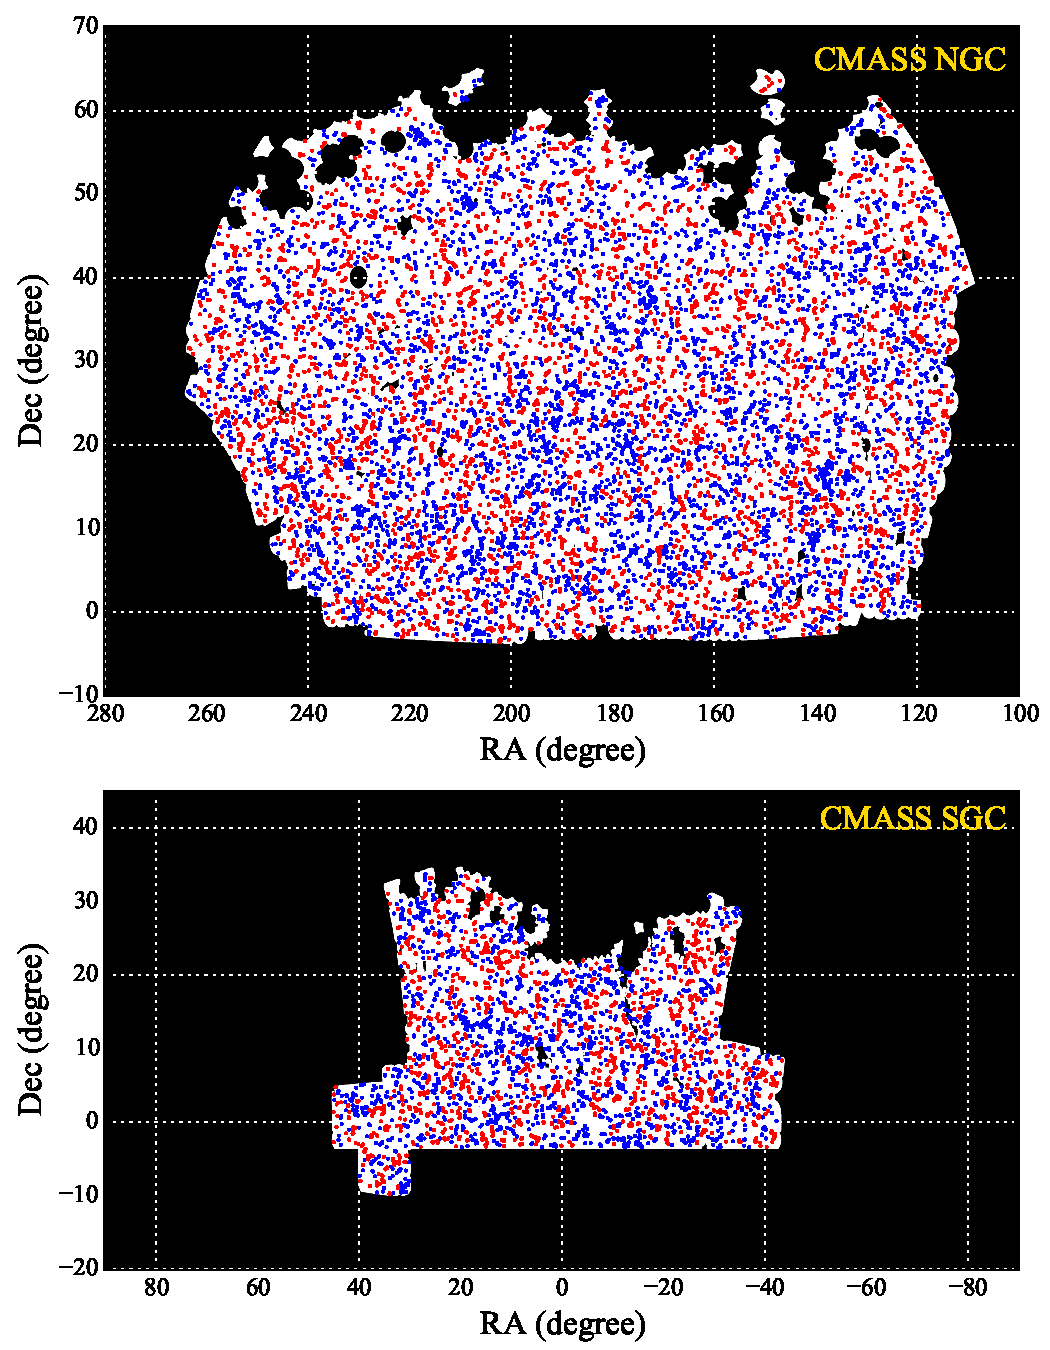
\includegraphics[width=.9\textwidth]{skyc}
\caption{BOSS DR11 CMASS NGC(上图)和SGC(下图)中,LRG(红色标记)和用LRG找到的半径$R \geq 16$ $h^{-1}$ Mpc的巨洞中心位置在天球上(RA,DEC)方向的投影。黑色的区域不能被有效观测,巨洞中心如果位于黑色区域那么该巨洞会被从样本中移除。可以看到巨洞的中心分布在没有LRG的区域内。(文献 ~\inlinecite{Kitaura2016Void} 中的FIG. 3)}
\label{fig:sky}
\end{figure}

这一节我们使用BOSS/SDSS-III CMASS DR11样本中红移$0.45 < z < 0.65$的NGC和SGC数据,并按照第~\ref{sec:lcdata} 章介绍的方法通过DIVE寻找真实观测数据中的巨洞。因为我们允许巨洞互相重叠,所以最终巨洞的数密度要大于星系的数密度,DR11 CMASS NGC中有1,212,393个$R \geq 16$ $h^{-1}$ Mpc的巨洞,566940个星系;SGC中有472868个巨洞,188582个星系。如果不允许巨洞重叠,那么在NGC中只有48000个巨洞。图~\ref{fig:sky} 分别展示了NGC和SGC区域内,星系和半径$R \geq 16$ $h^{-1}$ Mpc的巨洞中心位置在天球上的投影。

计算观测数据的巨洞2PCF前需要为其生成巨洞随机样本,与之前生成模拟光锥星系表的巨洞随机样本略有区别,具体方法如下:
\begin{description}
\item[1.] 将100个模拟光锥星系表中的巨洞数据合并起来得到合并数据。
\item[2.] 将合并数据按照红移分为$0.45 < z < 0.55$和$0.55 < z < 0.65$两组。
\item[3.] 将上面的两组数据再按半径不同分为如下五组,$16<R<17$、$17<R<18$、$18<R<19$、$19<R<20$、$20<R<50$ $h^{-1}$ Mpc。现在合并数据一共被分为10组。
\item[4.] 将每组数据分为球面坐标(RA,DEC)和红移与半径(z,R)两部分,只留下(RA,DEC)做为随机球面坐标。
\item[5.] 将观测数据的巨洞样本按照红移分为$0.45 < z < 0.55$和$0.55 < z < 0.65$两组,每组拆分为球面坐标(RA,DEC)和红移与半径(z,R)两部分,只留下(z,R)并将其复制十份,再按半径不同分为如下五组,$16<R<17$、$17<R<18$、$18<R<19$、$19<R<20$、$20<R<50$ $h^{-1}$ Mpc。
\item[6.] 将拆分后的十组(z,R)与对应的相同数量来自模拟光锥星系表巨洞数据的(RA,DEC)重新洗牌并随机组合。
\item[5.] 将十组随机洗牌后的数据合并成一组数据。
\end{description}

观测数据的巨洞随机样本准备好后,通过公式~(\ref{EQ:lsestimator})计算得到观测数据的巨洞2PCF。为了获得更准确的协方差矩阵,我们计算了1024个模拟光锥星系表的巨洞2PCF。第~\ref{sec:isobao} 章介绍了测量星系BAO特征尺度的方法,这里我们对此方法稍加改进,使其适用于测量巨洞的BAO信号。

公式~(\ref{EQ:xifit})中的$\xi_{m}$是基于线性理论推导得出的线性相关函数模型,而第~\ref{sec:voidbaocomplete} 章的结果表明巨洞的BAO信号有不同于星系BAO信号的一些特征,所以我们使用实空间完整模拟暗物质晕表的巨洞2PCF$\xi_{\rm w}$作为模版来构建测量巨洞BAO信号的模型$\xi_{\rm th}$。利用第~\ref{sec:datanw} 章的数据和DIVE可以得到没有BAO信号的巨洞数据,计算其中半径$R \geq 16$ $h^{-1}$ Mpc的巨洞2PCF可以得到没有BAO信号的巨洞2PCF$\xi_{\rm nw}$。所以,测量巨洞BAO信号的公式为(wiggle model):
\begin{equation}
\label{eq:isobaovoid}
\xi_{\rm th}(s) = B\,[\xi_{\rm w}(\alpha s) - \xi_{\rm nw}(s/\alpha)] + \xi_{\rm nw}(s/\alpha) + A(s)
\end{equation}
其中$\alpha$也同样表示基准宇宙学模型与真实观测值的比例,$B$表示BAO信号衰减的程度,$A(s)$与公式~(\ref{EQ:xifit})中的项相同,用于拟合除BAO信号外的整体形状,拟合区间为$60 < s < 160$ $h^{-1}$ Mpc。

为了测量BAO信号的显著性,我们也构建了一个不含BAO信号模型(nonwiggle model):
\begin{equation}
\xi_{\rm th}(s) = \xi_{\rm nw}(\alpha s) + A(s)
\end{equation}
这个模型等效于公式~(\ref{eq:isobaovoid})中$B = 0$的情况。

分别用以上两个模型拟合观测数据的巨洞2PCF,用第~\ref{sec:isobao} 章的方法得到协方差矩阵、$\chi^2$和似然函数。wiggle model的结果为$\chi^2/{\rm dof}=9.9/15$,nonwiggle model的结果为$\chi^2/{\rm dof}=20.1/16$,$\alpha$的最佳拟合值和$1\sigma$误差为$1.000 \pm 0.022$。在等效红移$z=0.57$处等价于$D_V = 2057 \pm 45$ Mpc,与星系的BAO测量结果一致$D_V = 2056 \pm 20$ Mpc。巨洞的$\chi^2$并不是非常符合高斯分布,但是仍然足够看作是一阶近似的结果,在未来的工作中将就这一问题作出改进。依据上述模型,我们使用观测数据的巨洞2PCF得到显著性为3.2 $\sigma$的BAO信号。RSD效应对巨洞BAO信号的影响可以被当作是阻尼项,这一项被包括在公式~(\ref{eq:isobaovoid})中的$B$中。图~\ref{fig:datadr11} 中展示了真数观测数据的巨洞2PCF、模拟光锥星系表的巨洞2PCF,wiggle model和nonwiggle model的最佳拟合。模拟光锥星系表的巨洞2PCF可以被认为是对观测数据的巨洞2PCF的理论预期。

DR11 CMASS的模拟光锥星系表模仿了真实观测数据中存在的各种问题,例如样本的不完备,天球部分区域不能被观测到(veto mask),两根光纤的最近距离不小于$55^{\prime\prime}$造成一些星系无法被观测到(fiber collision)。这些问题同也都存在于模拟光锥星系表的巨洞数据里。但是在巨洞的2PCF中并不存在严重的系统性偏差,可以看到图~\ref{fig:datadr11} 中观测数据的巨洞2PCF与模拟光锥星系表的理论预期非常接近,而文献 ~\inlinecite{Ross2012,Chuang2016}中观测数据的星系2PCF在较大距离处与模拟光锥星系表的理论预期存在非常大的偏差,需要给星系加上各种权重来减少系统性偏差。另一方面,虽然不同红移处星系的数密度不同会使巨洞的数密度随红移发生改变,但是我们选用半径$R \geq 16$ $h^{-1}$ Mpc的巨洞其数密度在不同红移处变化很小,这与第~\ref{sec:voidnumberdensity} 章的结果一致。

%图 巨洞不同红移处的数密度

\begin{figure}
\begin{tabular}{c}
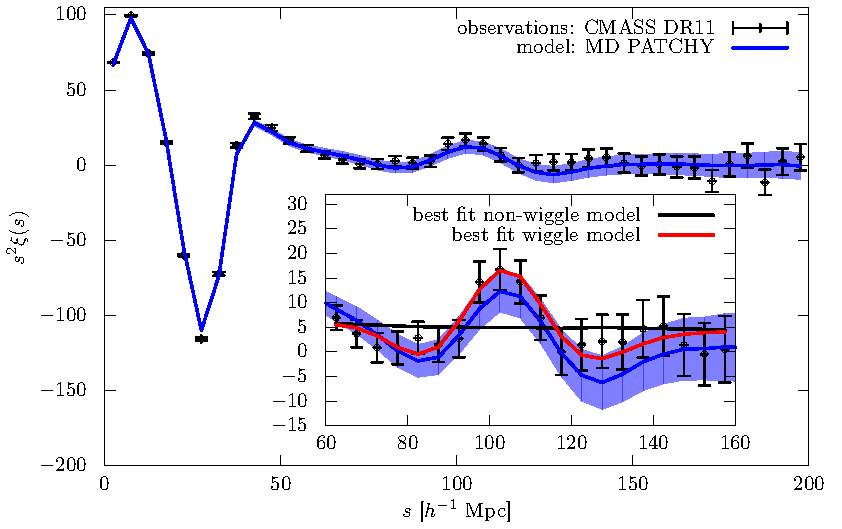
\includegraphics[width=.9\textwidth]{datad}
\put(-205,55){ 3.2 $\sigma$ detection}
\end{tabular}
\caption{ 红移$0.45 < z < 0.65$范围内,BOSS CMASS DR11 NGC和SGC样本(CMASS DR11)合在一起的巨洞2PCF(黑色误差棒),和用1024个BOSS CMASS DR11NGC和SGC的模拟光锥星系表(\textsc{MultiDark PATCHY},\textsc{MD PATCHY})的巨洞2PCF得到的平均值(蓝色实线)及1-$\sigma$范围内的理论预期(蓝色阴影)。红色实线与黑色实线分别是wiggle model与nonwiggle model的最佳拟合结果。(文献 ~\inlinecite{Kitaura2016Void} 中的FIG. 4)}
\label{fig:datadr11}
\end{figure}

%
%
%Question arise when we measure the clustering of voids: What is the information gain from void tracers directly computed from the distribution of galaxies? And how covariant are these tracers  to the galaxies themselves?
%The construction of void troughs follows the intuitive physical picture of filling the gaps complementary to the high density peaks occupied by the galaxies. Luminous red galaxies (LRGs) are known to reside in high density regions (see, e.g., Ref.~\citep[][]{KGS15}). We are thus, extending the information on the density fluctuations ($\delta=\rho/\bar{\rho}-1$) to underdense regions ($\delta<0$), which based on this galaxy distribution are otherwise set to a constant value ($\delta=-1$). { Less massive objects, such as emission line galaxies,  could also be used to define underdense regions, but
%an extended definition with some stellar mass threshold may be required for the estimation of troughs.}
%We note, that small voids are equivalent to groups of quartets of galaxies residing in high density regions (see Ref.~\citep[][]{2015arXiv151104299Z}), and, hence, are expected to deliver redundant information to the galaxies themselves.
%This is not the case for the large voids considered in this study. 
%In fact, it is clear, that the Delaunay voids we construct from tetrahedra of galaxies encode higher order statistics, further constrained by imposing the circumspheres to be empty, which strongly depends on gravitational evolution of the morphology of the cosmic web and hence, on all the $n$-point statistics of the density field (in particular the three-point statistics, see Ref.~\citep[][]{Frieman1994}). Moreover, our prior knowledge on the radius cut selecting empty circumspheres located in expanding void regions, based on tidal field computations of the underlying dark matter field in simulations (see Zhao {\it et~al.} companion paper \citep[][]{2015arXiv151104299Z}), implicitly incorporates knowledge on the void regions beyond  the one present in the galaxy distribution.
%By analyzing the clustering of the troughs (constructed upon the galaxies) we are including higher order information (see \citep[][]{W79}),  potentially circumventing a more complicated mathematical formalism needed to extract the full information encoded in the three-dimensional distribution of galaxies.
%This is supported by recent theoretical work, demonstrating that most of the information gained in BAO reconstruction comes from the three-point statistics with some contributions from the four-point statistics (see Ref.~\citep[][]{2015PhRvD..92l3522S}), and depends on the environment (see Ref.~\citep[][]{2015PhRvD..92h3523A}). In fact a recent work has presented a 2.8 $\sigma$ detection of BAOs from the three-point correlation function based on BOSS DR12 (see Ref.~\citep[][]{2015arXiv151202231S}). } 
%The actual information gain we can get from combining void tracers with galaxies in a multitracer analysis remains to be investigated, including whether voids will improve the cosmological constraints from galaxy clustering alone. This analysis may yield little added value in the presence of data covering the underdense cosmic density field, with, e.g., considerably higher number densities, than that provided by LRGs. 
%Nevertheless,  since  void tracers are expected to be less affected by gravitational pull,  BAO reconstruction techniques (see Ref.~\citep[][]{ESS07}) could be less necessary for these tracers, and they may thus yield a less cosmology-dependent estimate of the linear correlation function. We will investigate this in future work. 



%\section{BOSS/SDSS-III CMASS DR12样本的巨洞BAO信号}
%\label{sec:dr12}

%The first study will be done by using 100 Patchy mock halo catalogues in real space and redshift space. The real space void catalogues are constructed by running DIVE in the real space mock halo catalogues and the redshift space void catalogues are the products of running DIVE in the redshift space mock halo catalogues. 

%It is important to note that the redshift space void catalogues are not the transformation of the real space void catalogues by adding the redshift space distortion effect based on the velocity of the voids. In our definition, voids are the largest empty spheres defined by four nearest halos/galaxies. Even though there are ways to define the velocity of voids and use the velocity to make the transformation from real space to redshift space, the transformed redshift space voids are not necessarily empty of halos/galaxies, which is not consistent with our void definition. Our final goal is to apply our study on the observed galaxies data, which is in redshift space along with many other observation-related systematical effects. It is impossible to get the ideal real space galaxies catalogue of the Universe, so we need to make sure that our void finder and our method of measuring BAO with void catalogues are valid for redshift space data and observed data.

%I will first measure the BAO signal from the real space void catalogues and then move to redshift space void catalogues. Their difference is caused by the RSD effect of the halos. The voids are the tracers of the under dense regions in the universe, so the halos/galaxies around the boundary of the large voids will most probably move outside of the voids. This makes the under dense region enlarged from real space to redshift space along the line of sight. Since we keep our void definition as largest empty spheres devoid of halo/galaxy in both real space and redshift space, the real voids in redshift space will systematically be larger than the voids in real space but the clustering properties will not be significantly affected for voids in redshift space. Real voids trace the under dense regions. DIVE can find all the largest empty spheres but not all of them are really tracing the under dense regions. The radii of the DT voids could be very small if the four nearest halos/galaxies are happen located in a cluster. And the small voids found by DIVE are actually the tracers of denser regions, which correspond to groups (voids-in-clouds). So a proper way is needed to select the large voids which are the estimates of the troughs of the density field \textit{voids-in-voids}, from the whole sample of DT voids. Different aspects of void properties, including void number density, the density profile, the 2 points correlation function and power spectra, will be studied to make a proper distinction between of the large voids and small voids. 


%As described in ~\ref{sec:DIVE}, DIVE is a parameter free void finder and the only parameter for the DT voids is the radius. So the radius should be used to classify the large voids and the small voids. And there is one optimal void radius cut to select the large voids, whose radii are larger than the optimal radius, as the estimates of the troughs of the density field. The BAO signal, from the large voids selected by this optimal radius cut, is expected to be most significant than other radius cuts. And the optimal radius should also be a demarcation for other void properties to classify the large voids and the small voids.

%\subsection{BAO from voids in mock galaxies light-cone catalogues}

%I will investigate the measurement of BAO from the voids in the light-cone galaxy mock catalogues which encode redshift evolution from 0.45 to 0.65, the light-cone survey geometry, and other survey-related systematics effects. To validate the technique for measuring BAO of voids on observational data, the study will be performed on the Patchy galaxy mock light-cone catalogues which are specifically constructed for BOSS/SDSS CMASS DR11 galaxy catalogues. 

%The light-cone galaxy mocks are different from the redshift space halo mocks in cubical volume. The redshift space halo mocks have a uniform halo number density on large scale and it is a snapshot for redshift 0.56, which means the halos in the whole volume are at the same redshift. But the light-cone mocks covers a redshift range from 0.4 to 0.7 along line of sight and there is a galaxy number density as a function of redshift (see Fig.~\ref{fig:AndersonFig1}). The galaxy number density at redshift 0.4 and 0.7 is relatively small so only the sample within 0.45 to 0.65 will be used in the study.

%The \citet{Peebles1974} estimator works fine with the mocks in cubic volume but it is not a good estimator for the light-cone mocks. For light-cone mocks, we use the \citet[][]{Landy1993} estimator:
%\begin{equation} \label{EQ:lsestimator}
%\xi (s)=\frac {DD(s)-2DR(s)+RR(s)} {RR(s)} \,,
%\end{equation}
%where $DD$ is the normalized data-data pair counts, $DR$ is the normalized data-random pair counts, and $RR$ correspond to the normalized random-random pair counts. There is no good analytical formula for the $DR$ and $RR$ terms of the light-cone mocks. So a random catalogue for computing the $DR$ and $RR$ terms is needed for the void light-cone mocks. Since the distribution of voids is different from the galaxy distribution, especially near the boundary of the survey, the galaxy random catalogue may not be suitable for computing the 2 point correlation function of the void catalogues. The void random catalogues will be constructed following the same method for constructing the galaxy random catalogues. And I will test if it is proper for the void mock catalogues.

%The 2PCF will be computed for different void subsamples with different radius cuts and radius bins to find again the optimal radius cut that gives the best BAO signal-to-noise ratio. There are many survey-related systematics effect on the light-cone mocks, so the optimal radius cut found by the light-cone mocks may not be the same as we found with the real space void mocks and the redshift space void mocks. But the difference should be small.

%\subsection{Measure void BAO from LRG sample of BOSS}

%The BOSS survey, comprised of the SDSS-III observations through 2013 May, achieved 1 percent measurement of the BAO characteristic acoustic scale in the clustering of galaxies. The CMASS LRG sample are selected from the DR8 imaging with a median redshift $z=0.57$~\cite{Dawson2013}. Most of the CMASS LRG targets are central galaxies of dark matter halos with mass larger than about $10^{13} M_{\odot}$ while a non-negligible fraction of the targets are satellites galaxies residing in dark matter halos about 10 times more massive ~\cite{White2011,Nuza2013}. This work will be done with the DR11 CMASS LRG sample of the BOSS survey. Even though the light-cone mocks are designed to reproduce the 2 point statistics from the observed DR11 and DR12 CMASS LRG sample, and have been randomly down-sampled to have the same mean $n(z)$ from the observed sample, there are still non-negligible difference between the observed data and the light-cone mocks. So a new random catalogue will be generated for computing the 2 point correlation function of the observed data. And the error of the 2PCF of the observed data will be estimated with the light-cone mocks.









